\documentclass[letter,12pt,bahasa]{article}
\author{Maleka Ghaniya \and Jorell Ramos Sinaga \and Angela Vania Sugiyono}
\date{}
\usepackage[a4paper, top=25mm, bottom=25mm, left=30mm, right=25mm]{geometry}

\usepackage[bahasa]{babel}
\usepackage[utf8]{inputenc}
\usepackage{amsmath,amssymb}
\usepackage{lscape}
\usepackage[colorinlistoftodos]{todonotes}
\usepackage{fancyhdr}
\usepackage[hidelinks]{hyperref}

\usepackage{graphicx}
\graphicspath{ {./} }

\usepackage{listings}
\usepackage{xcolor}
\usepackage{seqsplit}
\usepackage{float}
\usepackage{longtable}

\setlength{\parindent}{2em}
\setlength{\parskip}{0.5em}
\usepackage{indentfirst}

\usepackage{titlesec}

\titlespacing*{\subsection}
  {0pt}
  {1.5ex plus 0.5ex minus 0.5ex}
  {0.8ex}

\titlespacing*{\subsubsection}
  {0pt}
  {1.0ex plus 0.3ex minus 0.3ex}
  {0.6ex}

\usepackage{ragged2e}
\justifying

\usepackage{array}
\usepackage{booktabs}
\usepackage{adjustbox}
\usepackage{multirow}

\definecolor{codegreen}{rgb}{0,0.6,0}
\definecolor{codegray}{rgb}{0.5,0.5,0.5}
\definecolor{codepurple}{rgb}{0.58,0,0.82}
\definecolor{backcolour}{rgb}{0.95,0.95,0.92}

\lstdefinestyle{sql}{
    backgroundcolor=\color{backcolour},
    commentstyle=\color{codegreen},
    keywordstyle=\color{blue}\bfseries,
    numberstyle=\tiny\color{codegray},
    stringstyle=\color{codepurple},
    basicstyle=\ttfamily\footnotesize,
    breakatwhitespace=false,
    breaklines=true,
    captionpos=b,
    keepspaces=true,
    numbers=left,
    numbersep=5pt,
    showspaces=false,
    showstringspaces=false,
    showtabs=false,
    tabsize=4,
    language=SQL,
}

\renewcommand{\lstlistlistingname}{Daftar Listing}
\renewcommand{\lstlistingname}{Listing}

\pagestyle{fancy}
\fancyhf{}
\chead{Laporan Final Project --- Sistem Basis Data Bioskop CineTrack}
\cfoot{\thepage}

\begin{document}

% ============================================================
% COVER PAGE
% ============================================================
\begin{titlepage}
\begin{center}
    \vspace*{1cm}
 
    {\large \textbf{Laporan Final Project} \\[0.8cm]
    \textit{SISTEM BASIS DATA BIOSKOP CINETRACK:} \\[0.4cm]
    \large Perancangan, Implementasi, dan Analisis Normalisasi Basis Data Operasional Bioskop Multi-Cabang} \\[1.5cm]
 
    
\includegraphics[width=0.5\textwidth]{Lambang-ITS.png} \\[1.5cm]
 
    {\normalsize
    \begin{tabular}{ll}
        \multicolumn{2}{l}{\textbf{Anggota Kelompok:}} \\[0.3cm]
        Maleka Ghaniya        & 5025241189 \\[0.2cm]
        Jorell Ramos Sinaga   & 5025241202 \\[0.2cm]
        Angela Vania Sugiyono & 5025241226 \\
    \end{tabular}} \\[2cm]
 
    \vfill
    {\large Departemen Teknik Informatika, FTEIC \\
    Institut Teknologi Sepuluh Nopember} \\[0.5cm]
    {\large 2026}
\end{center}
\end{titlepage}
 
\clearpage
 
\tableofcontents
\listoftables
\listoffigures
 
\clearpage

% ============================================================
% SECTION 1: STUDI KASUS
% ============================================================
\section{Studi Kasus}

\subsection{Latar Belakang}

CineTrack adalah bioskop lokal yang telah beroperasi lebih dari satu dekade, namun hingga kini seluruh proses operasionalnya, penjualan tiket, pencatatan jadwal tayang, hingga pemantauan stok kantin masih dikelola secara manual. Seiring bertambahnya jumlah pengunjung dan studio, cara ini mulai menimbulkan masalah serius seperti kursi terjual ganda karena tidak ada sinkronisasi antar kasir, laporan pendapatan harian sulit disusun karena data tersebar di berbagai catatan terpisah, dan manajemen tidak memiliki gambaran yang jelas tentang status penayangan film untuk keperluan promosi. Oleh karena itu, manajemen CineTrack memutuskan untuk membangun sistem basis data terpusat yang mengintegrasikan seluruh kebutuhan operasional bioskop. Lebih dari itu, CineTrack yang awalnya beroperasi sebagai bioskop tunggal kini tengah merencanakan ekspansi dengan membuka cabang di beberapa kota besar di Indonesia. Untuk mendukung pertumbuhan ini, sistem basis data yang dirancang perlu mengakomodasi pengelolaan multi-cabang, di mana setiap cabang memiliki studio, jadwal tayang, dan operasional tersendiri namun tetap terintegrasi dalam satu sistem terpusat milik manajemen pusat CineTrack.

\subsection{Studio dan Film}

Bioskop ini memiliki beberapa studio, masing-masing dengan kapasitas berbeda dan kursi yang dibagi ke dalam tipe reguler, VIP, dan \textit{couple seat}, tiap tipe memiliki tarif sendiri dan posisi kursi dicatat berdasarkan baris dan kolom. Setiap film yang ditayangkan menyimpan informasi seperti judul, genre, durasi, rating usia, sinopsis, sutradara, dan pemeran utama, serta memiliki status penayangan yang dapat berubah antara \textit{coming soon}, \textit{now showing}, dan \textit{leaving soon}, status ini digunakan oleh tim promosi sebagai dasar pembuatan poster dan materi iklan.

\subsection{Jadwal Tayang}

Setiap hari disusun jadwal tayang yang menentukan film mana ditayangkan di studio mana, pada tanggal dan jam berapa; satu studio dapat memiliki beberapa sesi dalam sehari dengan film yang berbeda. Harga dasar tiket per sesi dapat bervariasi tergantung waktu tayang dan hari. Sesi malam dan akhir pekan umumnya dikenakan tarif lebih tinggi.

\subsection{Transaksi dan Pembayaran}

Saat pelanggan datang ke loket, kasir menampilkan peta kursi yang tersedia untuk sesi yang dipilih; pelanggan dapat memesan satu atau lebih kursi sekaligus dan menambahkan pembelian makanan atau minuman kantin dalam transaksi yang sama, di mana setiap produk kantin memiliki nama, kategori, harga satuan, dan stok tercatat. Total tagihan merupakan akumulasi harga tiket dan produk kantin; pembayaran dapat dilakukan tunai maupun non-tunai. Data pelanggan seperti nama, nomor telepon, dan surel ikut dicatat, begitu pula identitas kasir yang menangani transaksi beserta \textit{shift} kerjanya.

\subsection{Kebutuhan Laporan}

Pada akhir hari, manajer membutuhkan laporan yang merangkum total pendapatan tiket per studio dan per film, jumlah kursi terisi per sesi tayang, serta produk kantin paling laris; riwayat transaksi per pelanggan juga perlu tersimpan sebagai dasar program loyalitas ke depannya. Berdasarkan seluruh kebutuhan ini, manajemen CineTrack menugaskan tim untuk merancang dan mengimplementasikan sistem basis data yang mencakup perancangan struktur data, \textit{query} pelaporan, fungsi kalkulasi otomatis, serta prosedur transaksi yang aman dan konsisten.

\clearpage

% ============================================================
% SECTION 2: PERANCANGAN BASIS DATA
% ============================================================
\section{Perancangan Basis Data}

\subsection{Entity Relationship Diagram (ERD)}

ERD pada tahap ini merupakan model logis yang merepresentasikan entitas, atribut, dan relasi antar entitas secara konseptual tanpa mempertimbangkan implementasi fisik. Terdapat 14 entitas utama yang saling berelasi, yaitu \texttt{cabang}, \texttt{studio}, \texttt{kursi}, \texttt{film}, \texttt{genre}, \texttt{jadwal\_tayang}, \texttt{tiket}, \texttt{transaksi}, \texttt{pelanggan}, \texttt{pegawai}, \texttt{shift}, \texttt{pembayaran}, \texttt{produk\_kantin}, dan \texttt{kategori}. Relasi \textit{many-to-many} antar entitas seperti film--genre, jadwal--film, pegawai--shift, dan transaksi--produk kantin pada tahap ini masih direpresentasikan sebagai relasi langsung dengan kardinalitas N:N, dan baru akan ditransformasikan menjadi tabel \textit{junction} pada tahap PDM.

\begin{figure}[H]
    \centering
    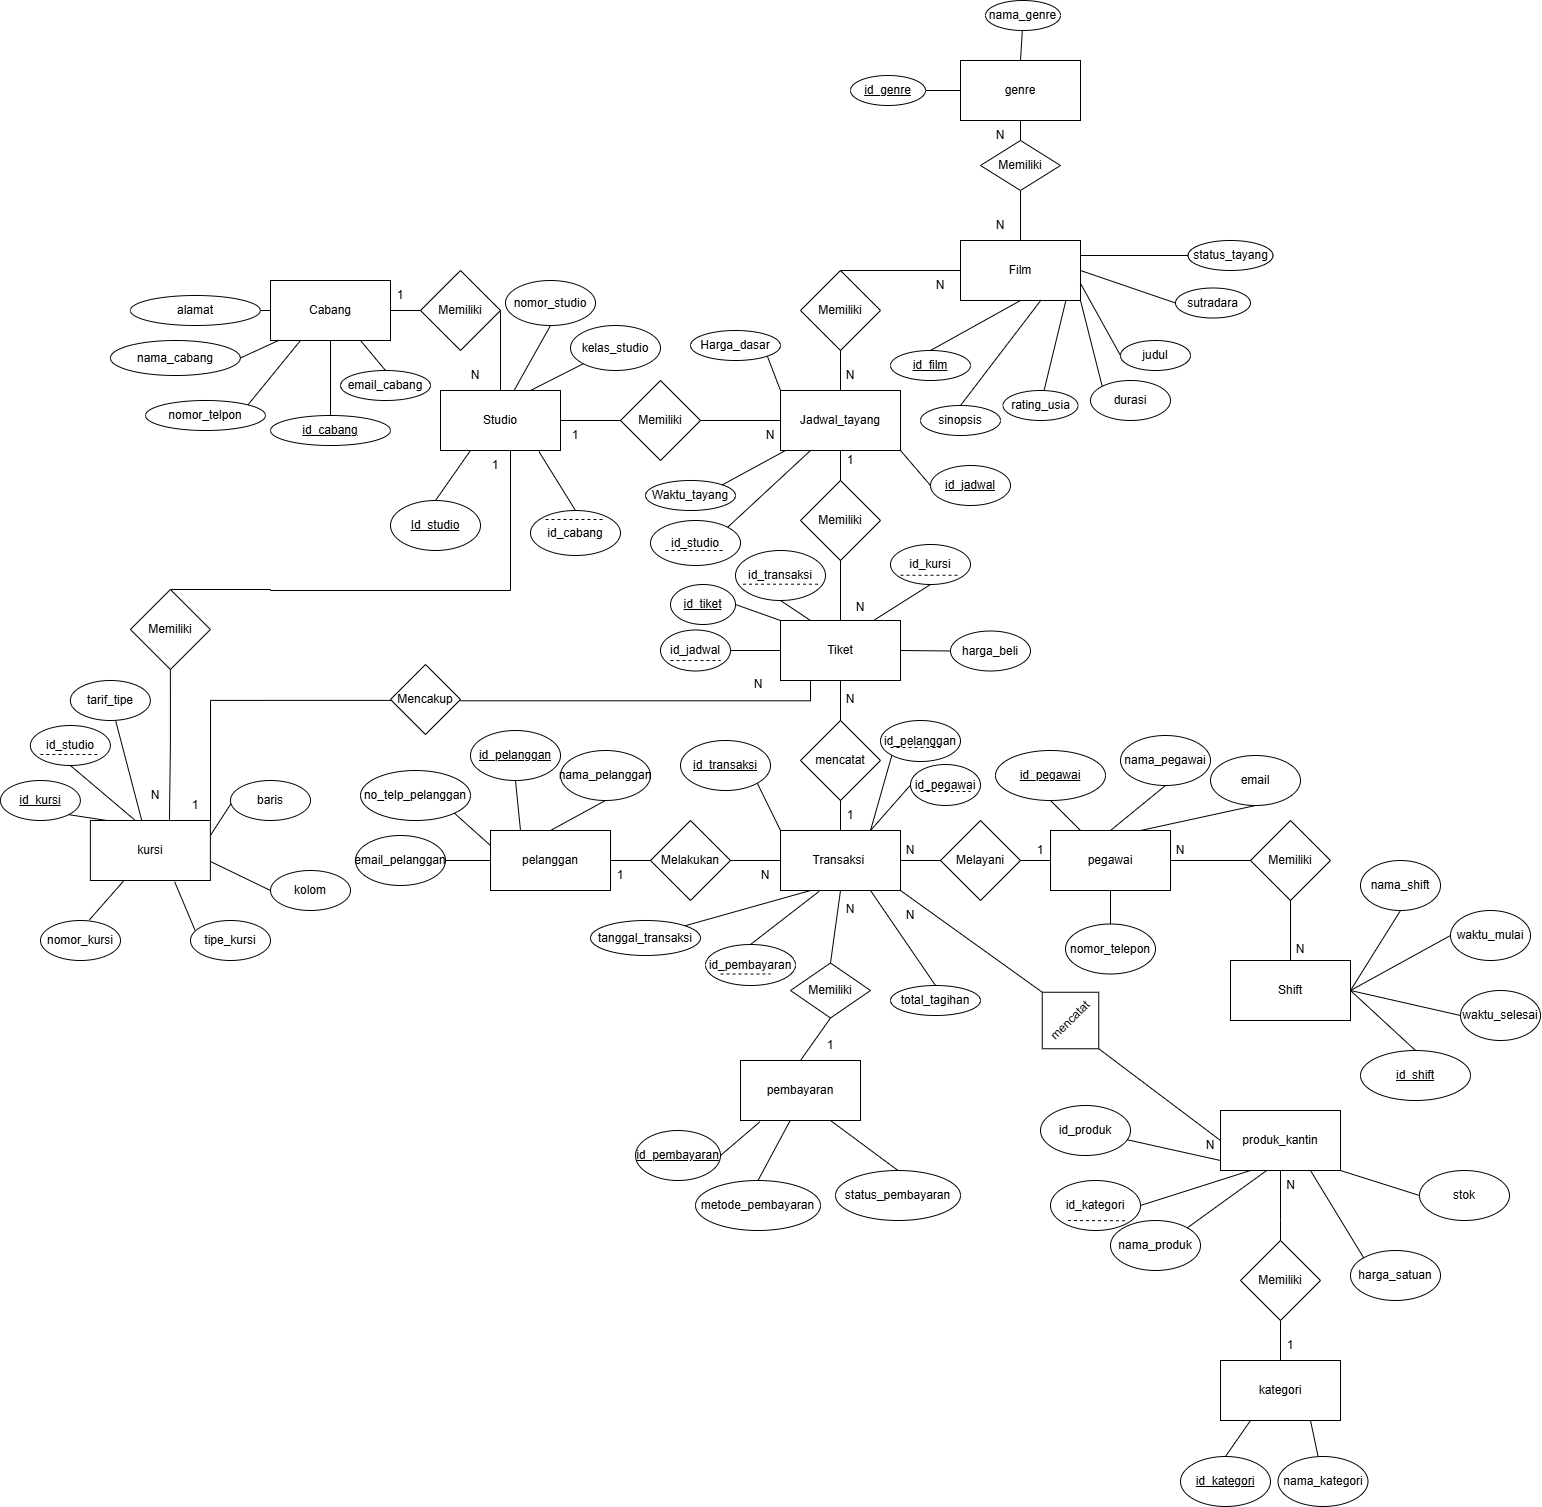
\includegraphics[width=0.95\linewidth]{tugas-fp/erd_fp_mbd_fiks.png}
    \caption{ERD Sistem Basis Data Bioskop CineTrack}
    \label{fig:erd_cinetrack}
\end{figure}

\subsection{Conceptual Data Model (CDM)}

CDM merepresentasikan struktur data pada tingkat konseptual menggunakan notasi Redgate Data Modeler. Pada tahap ini, 14 entitas ditampilkan beserta atribut dan kardinalitas relasinya. Relasi \textit{many-to-many} seperti film--genre, jadwal--film, pegawai--shift, dan transaksi--produk kantin masih direpresentasikan sebagai relasi langsung antar entitas tanpa tabel \textit{junction}, sesuai dengan sifat model konseptual yang belum menyentuh detail implementasi fisik.

\begin{figure}[H]
    \centering
    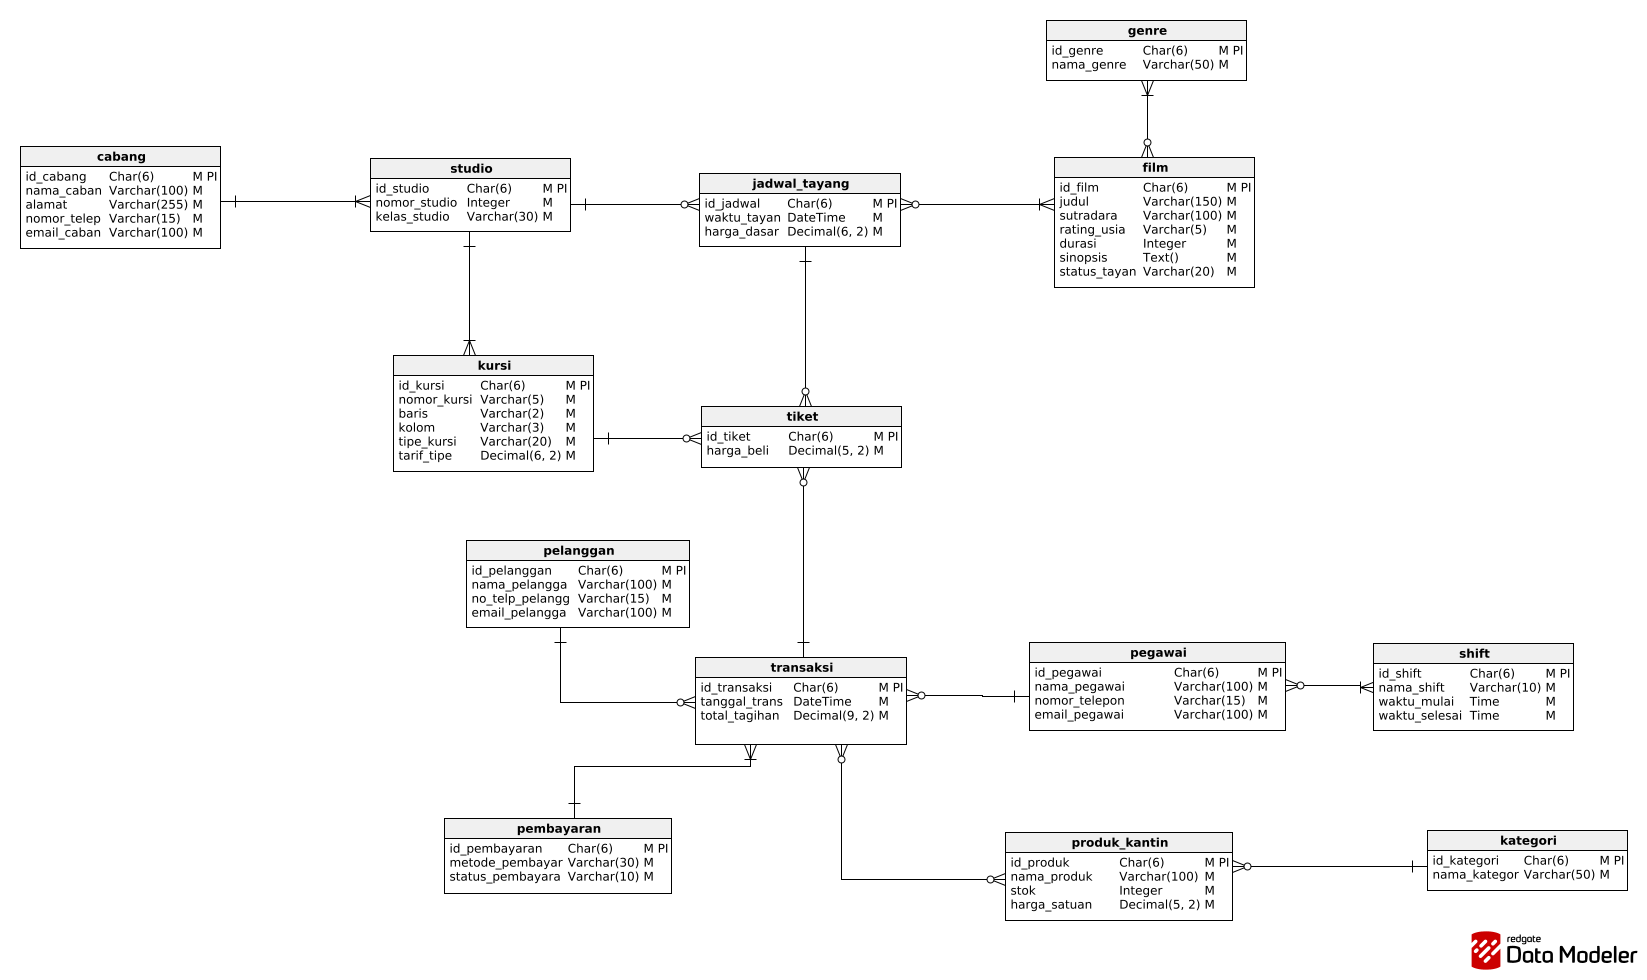
\includegraphics[width=0.95\linewidth]{tugas-fp/cdm_fp_mbd_fiks.png}
    \caption{CDM Sistem Basis Data Bioskop CineTrack}
    \label{fig:cdm_cinetrack}
\end{figure}

\subsection{Physical Data Model (PDM)}

PDM merupakan hasil transformasi CDM ke dalam bentuk fisik yang siap diimplementasikan pada sistem manajemen basis data. Pada tahap ini, seluruh relasi \textit{many-to-many} ditransformasikan menjadi tabel \textit{junction} eksplisit, yaitu \texttt{film\_genre}, \texttt{jadwal\_tayang\_film}, \texttt{pegawai\_shift}, dan \texttt{produk\_kantin\_transaksi}. Seluruh \textit{foreign key} dan tipe data juga telah didefinisikan secara eksplisit, sehingga total terdapat 18 tabel pada PDM.

\begin{figure}[H]
    \centering
    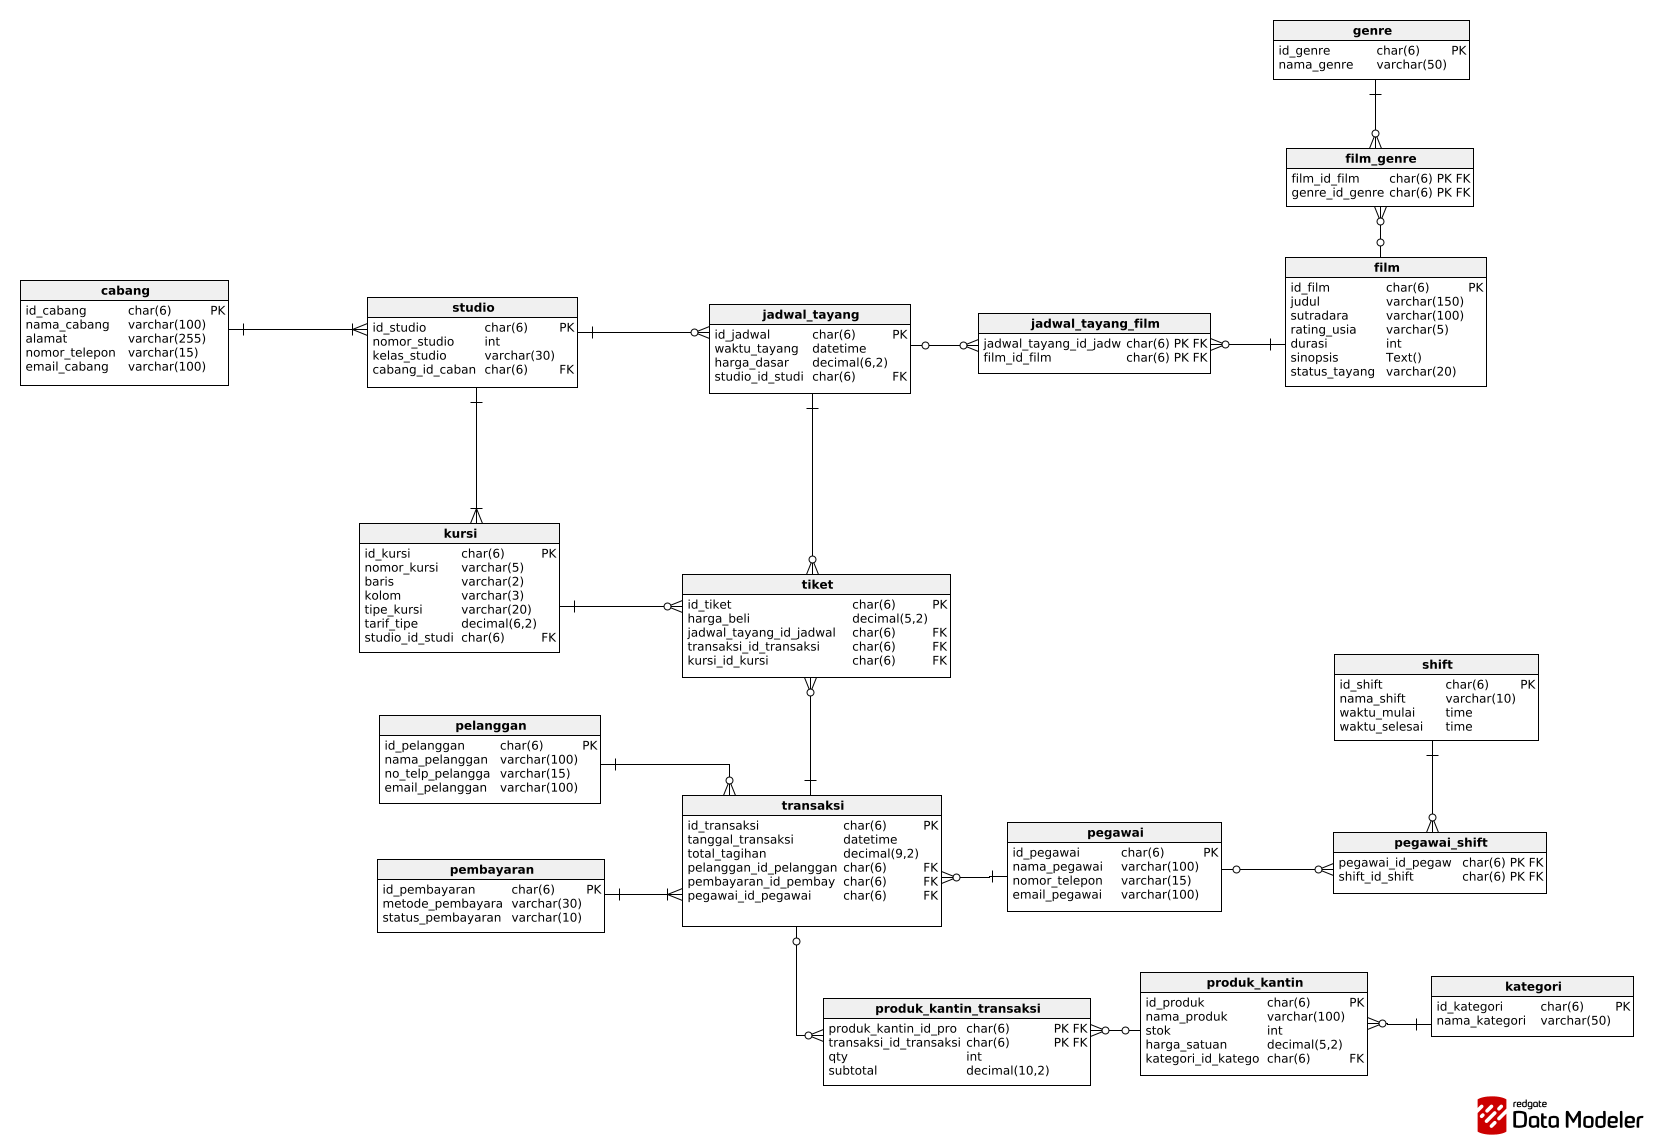
\includegraphics[width=0.95\linewidth]{tugas-fp/pdm_fp_mbd_fiks.png}
    \caption{PDM Sistem Basis Data Bioskop CineTrack}
    \label{fig:pdm_cinetrack}
\end{figure}

\clearpage

% ============================================================
% SECTION 3: NORMALISASI 3NF
% ============================================================
\section{Analisis Normalisasi hingga Bentuk Normal Ketiga (3NF)}

\subsection{Definisi 3NF}

Suatu relasi dikatakan berada dalam Bentuk Normal Ketiga (3NF) apabila memenuhi tiga syarat berikut:
\begin{enumerate}
    \item Berada dalam 1NF: setiap atribut bernilai atomik dan tidak ada grup atribut yang berulang.
    \item Berada dalam 2NF: setiap atribut non-\textit{key} bergantung secara penuh pada \textit{primary key} (tidak ada \textit{partial dependency}).
    \item Tidak terdapat \textit{transitive dependency}: atribut non-\textit{key} tidak bergantung pada atribut non-\textit{key} lainnya.
\end{enumerate}

\subsection{Analisis Per Tabel}

Berikut adalah analisis pemenuhan 3NF untuk setiap tabel pada basis data CineTrack.

\begin{longtable}{|c|p{2.9cm}|p{3.5cm}|p{5.8cm}|c|}
\caption{Analisis Normalisasi 3NF Basis Data CineTrack}
\label{tab:normalisasi_3nf} \\
\hline
\textbf{No} & \textbf{Tabel} & \textbf{Primary Key} & \textbf{Atribut Non-Key} & \textbf{3NF} \\
\hline
\endfirsthead
\hline
\textbf{No} & \textbf{Tabel} & \textbf{Primary Key} & \textbf{Atribut Non-Key} & \textbf{3NF} \\
\hline
\endhead
\hline
\multicolumn{5}{r}{\textit{(bersambung ke halaman berikutnya)}} \\
\endfoot
\hline
\endlastfoot
1 & \texttt{cabang} & \texttt{id\_cabang} & \texttt{nama\_cabang, alamat, nomor\_telepon, email\_cabang} --- semua bergantung penuh pada \texttt{id\_cabang}, tidak ada dependensi transitif. & \checkmark \\
\hline
2 & \texttt{studio} & \texttt{id\_studio} & \texttt{nomor\_studio, kelas\_studio} --- bergantung penuh pada \texttt{id\_studio}. FK \texttt{cabang\_id\_cabang} merupakan referensi eksternal, bukan dependensi transitif. & \checkmark \\
\hline
3 & \texttt{kursi} & \texttt{id\_kursi} & \texttt{nomor\_kursi, baris, kolom, tipe\_kursi, tarif\_tipe} --- semua bergantung penuh pada \texttt{id\_kursi}. \texttt{tarif\_tipe} adalah tarif per tipe kursi yang merupakan properti intrinsik kursi, bukan atribut yang bergantung pada atribut non-\textit{key} lain. & \checkmark \\
\hline
4 & \texttt{jadwal\_tayang} & \texttt{id\_jadwal} & \texttt{waktu\_tayang, harga\_dasar} --- keduanya merupakan properti sesi tayang yang bergantung penuh pada \texttt{id\_jadwal}. Tidak ada dependensi transitif. & \checkmark \\
\hline
5 & \texttt{film} & \texttt{id\_film} & \texttt{judul, durasi, sinopsis, rating\_usia, sutradara, status\_tayang} --- semua bergantung penuh pada \texttt{id\_film}. Genre dipisah ke tabel \texttt{film\_genre} untuk menghindari redundansi. & \checkmark \\
\hline
6 & \texttt{genre} & \texttt{id\_genre} & \texttt{nama\_genre} --- bergantung penuh pada \texttt{id\_genre}. & \checkmark \\
\hline
7 & \texttt{film\_genre} & \texttt{film\_id\_film,} \newline \texttt{genre\_id\_genre} \newline (komposit) & Tidak ada atribut non-\textit{key}. Tabel \textit{junction} murni untuk relasi \textit{many-to-many} film--genre. & \checkmark \\
\hline
8 & \texttt{jadwal\_tayang\_\newline}film & \texttt{jadwal\_tayang\_\newline}id\_jadwal, \newline \texttt{film\_id\_film} \newline (komposit) & Tidak ada atribut non-\textit{key}. Tabel \textit{junction} untuk relasi \textit{many-to-many} jadwal--film. & \checkmark \\
\hline
9 & \texttt{tiket} & \texttt{id\_tiket} & \texttt{harga\_beli} --- merupakan \textit{snapshot} harga saat transaksi terjadi, bergantung pada \texttt{id\_tiket}. FK \texttt{id\_jadwal}, \texttt{id\_transaksi}, \texttt{id\_kursi} adalah referensi eksternal. & \checkmark \\
\hline
10 & \texttt{pelanggan} & \texttt{id\_pelanggan} & \texttt{nama\_pelanggan, no\_telp\_pelanggan, email\_pelanggan} --- semua bergantung penuh pada \texttt{id\_pelanggan}. & \checkmark \\
\hline
11 & \texttt{pegawai} & \texttt{id\_pegawai} & \texttt{nama\_pegawai, nomor\_telepon, email\_pegawai} --- semua bergantung penuh pada \texttt{id\_pegawai}. & \checkmark \\
\hline
12 & \texttt{shift} & \texttt{id\_shift} & \texttt{nama\_shift, waktu\_mulai, waktu\_selesai} --- bergantung penuh pada \texttt{id\_shift}. & \checkmark \\
\hline
13 & \texttt{pegawai\_shift} & \texttt{pegawai\_id\_pegawai,} \newline \texttt{shift\_id\_shift} \newline (komposit) & Tidak ada atribut non-\textit{key}. Tabel \textit{junction} untuk relasi \textit{many-to-many} pegawai--shift. & \checkmark \\
\hline
14 & \texttt{pembayaran} & \texttt{id\_pembayaran} & \texttt{metode\_pembayaran, status\_pembayaran} --- bergantung penuh pada \texttt{id\_pembayaran}. & \checkmark \\
\hline
15 & \texttt{transaksi} & \texttt{id\_transaksi} & \texttt{tanggal\_transaksi, total\_tagihan} --- bergantung penuh pada \texttt{id\_transaksi}. \texttt{total\_tagihan} disimpan sebagai \textit{snapshot} akumulasi untuk keperluan audit, bukan \textit{derived attribute} yang dihitung ulang. & \checkmark \\
\hline
16 & \texttt{produk\_kantin} & \texttt{id\_produk} & \texttt{nama\_produk, stok, harga\_satuan} --- bergantung penuh pada \texttt{id\_produk}. Kategori dipisah ke entitas \texttt{kategori} untuk menghindari redundansi nilai berulang. & \checkmark \\
\hline
17 & \texttt{kategori} & \texttt{id\_kategori} & \texttt{nama\_kategori} --- bergantung penuh pada \texttt{id\_kategori}. & \checkmark \\
\hline
18 & \texttt{produk\_kantin\_\newline}transaksi & \texttt{produk\_kantin\_\newline}id\_produk, \newline \texttt{transaksi\_id\_\newline}transaksi \newline (komposit) & \texttt{qty} (INT) dan \texttt{subtotal} (DECIMAL(10,2)) --- keduanya bergantung penuh pada kombinasi PK komposit. \texttt{subtotal} merupakan \textit{snapshot} hasil \texttt{qty} $\times$ \texttt{harga\_satuan} saat transaksi. & \checkmark \\
\end{longtable}

\subsection{Keputusan Desain yang Mendukung 3NF}

Beberapa keputusan desain penting yang dilakukan untuk memastikan pemenuhan 3NF adalah sebagai berikut:

\subsubsection{Pemisahan Entitas \texttt{genre} dari \texttt{film}}
Apabila \texttt{genre} disimpan sebagai atribut Varchar langsung di \texttt{film}, nilai seperti ``Action'' akan berulang di banyak baris --- melanggar prinsip minimasi redundansi. Lebih lanjut, satu film dapat memiliki lebih dari satu genre (\textit{many-to-many}), sehingga diperlukan tabel \textit{junction} \texttt{film\_genre} dengan PK komposit (\texttt{film\_id\_film}, \texttt{genre\_id\_genre}).

\subsubsection{Pemisahan Entitas \texttt{kategori} dari \texttt{produk\_kantin}}
Serupa dengan genre, nilai kategori produk kantin (seperti ``Makanan'' dan ``Minuman'') akan berulang di setiap baris tabel \texttt{produk\_kantin} apabila disimpan sebagai Varchar. Dengan memisahkannya ke entitas \texttt{kategori}, redundansi dieliminasi dan konsistensi nilai terjaga.

\subsubsection{Tabel \textit{Junction} \texttt{produk\_kantin\_transaksi}}
Satu transaksi dapat mencakup pembelian banyak produk kantin dengan kuantitas berbeda-beda. Apabila \texttt{id\_produk} disimpan langsung sebagai FK di \texttt{transaksi}, hanya satu produk yang dapat dicatat per transaksi. Tabel \textit{junction} ini memungkinkan pencatatan \texttt{qty} dan \texttt{subtotal} per produk per transaksi, sekaligus memenuhi 2NF karena kedua atribut tersebut bergantung penuh pada kombinasi PK komposit.

\subsubsection{Atribut \textit{Snapshot}: \texttt{harga\_beli} dan \texttt{subtotal}}
Nilai \texttt{harga\_beli} pada \texttt{tiket} dan \texttt{subtotal} pada \texttt{produk\_kantin\_transaksi} secara konseptual bersifat \textit{derived}, namun sengaja disimpan sebagai atribut fisik. Hal ini dilakukan untuk menjaga integritas data historis --- apabila \texttt{tarif\_tipe} atau \texttt{harga\_satuan} berubah di kemudian hari, harga yang telah dibayarkan tetap tercatat dengan benar. Pendekatan ini tidak melanggar 3NF karena nilai-nilai tersebut bergantung penuh pada PK tabelnya masing-masing.

\subsubsection{Pemisahan Relasi \texttt{pegawai}--\texttt{shift} menjadi \textit{Many-to-Many}}
Seorang pegawai dapat bertugas pada shift yang berbeda di hari yang berbeda, dan satu shift dapat diisi oleh banyak pegawai. Oleh karena itu, relasi ini dimodelkan sebagai \textit{many-to-many} melalui tabel \textit{junction} \texttt{pegawai\_shift}, menghindari redundansi data shift yang akan terjadi apabila disimpan langsung di entitas \texttt{pegawai}.

\subsection{Kesimpulan Normalisasi}

Seluruh 18 tabel pada basis data CineTrack telah memenuhi Bentuk Normal Ketiga (3NF). Tidak ditemukan \textit{partial dependency} maupun \textit{transitive dependency} pada struktur yang dirancang. Desain ini memastikan data tersimpan secara efisien, konsisten, dan mudah dipelihara seiring bertambahnya skala operasional CineTrack.

\clearpage

% ============================================================
% SECTION 4: IMPLEMENTASI SQL DAN DATA RECORD
% ============================================================
\section{Implementasi SQL dan Data Record}

Implementasi basis data CineTrack dilakukan pada MySQL menggunakan database bernama \texttt{MBD\_FP}. Seluruh tabel dibuat menggunakan perintah DDL sesuai PDM yang telah dirancang, kemudian diisi dengan data \textit{seed} sebanyak 20 \textit{record} pada setiap tabel utama. Berikut adalah catatan penting terkait implementasi:

\begin{itemize}
    \item Tipe data kolom harga (\texttt{tarif\_tipe}, \texttt{harga\_dasar}, \texttt{harga\_beli}, \texttt{harga\_satuan}) direvisi dari \texttt{DECIMAL(6,2)} dan \texttt{DECIMAL(5,2)} menjadi \texttt{DECIMAL(10,2)} untuk mengakomodasi nilai harga dalam satuan rupiah yang dapat mencapai ratusan ribu. Revisi ini merupakan koreksi terhadap PDM awal yang tidak mempertimbangkan skala mata uang rupiah.
    \item Tiga pelanggan tambahan (\texttt{PL0021}--\texttt{PL0023}) ditambahkan tanpa data transaksi untuk memenuhi kebutuhan Query Kasus 5 (pelanggan yang belum pernah bertransaksi).
    \item Nilai \texttt{harga\_beli} pada tabel \texttt{tiket} disimpan sebagai \textit{snapshot} pada saat transaksi dilakukan, sehingga perubahan tarif di masa mendatang tidak akan memengaruhi data historis.
\end{itemize}

\clearpage

% ============================================================
% SECTION 5: QUERY CASES
% ============================================================
\section{Implementasi SQL Query}

\subsection{Kasus Query pada Sistem CineTrack}

Berikut adalah lima studi kasus \textit{query} yang diimplementasikan pada basis data CineTrack, masing-masing merepresentasikan kebutuhan informasi nyata dalam operasional bioskop.

\begin{landscape}
\begin{longtable}{|c|p{3.0cm}|p{5.5cm}|p{12.0cm}|}
\caption{Kasus Query pada Sistem Basis Data CineTrack}
\label{tab:query_cases} \\
\hline
\textbf{No} & \textbf{Kasus} & \textbf{Kebutuhan Informasi} & \textbf{Aljabar Relasional} \\
\hline
\endfirsthead
\hline
\textbf{No} & \textbf{Kasus} & \textbf{Kebutuhan Informasi} & \textbf{Aljabar Relasional} \\
\hline
\endhead
\hline
\multicolumn{4}{r}{\textit{(bersambung ke halaman berikutnya)}} \\
\endfoot
\hline
\endlastfoot
1 & Menampilkan daftar film beserta genre-nya &
Tim promosi membutuhkan daftar film \textit{Now Showing} beserta genre untuk keperluan pembuatan materi iklan. &
$\pi_{\texttt{judul,\ status,\ nama\_genre}}\bigl(\sigma_{\texttt{status\_tayang}=\textit{`Now\ Showing'}}(\texttt{film}) \bowtie \texttt{film\_genre} \bowtie \texttt{genre}\bigr)$ \\
\hline
2 & Menampilkan jadwal tayang lengkap beserta film dan studio &
Kasir perlu menampilkan jadwal tayang hari ini lengkap dengan nama film, kelas studio, harga dasar, dan cabang kepada pelanggan. &
$\pi_{\texttt{waktu,\ film,\ kelas,\ harga\_dasar,\ cabang}}\bigl(\texttt{jadwal\_tayang} \bowtie \texttt{jadwal\_tayang\_film} \bowtie \texttt{film} \bowtie \texttt{studio} \bowtie \texttt{cabang}\bigr)$ \\
\hline
3 & Menampilkan transaksi dengan total tagihan di atas Rp200.000 &
Manajer ingin mengidentifikasi transaksi bernilai tinggi untuk analisis pola pembelian pelanggan premium. &
$\pi_{\texttt{id\_transaksi,\ pelanggan,\ total,\ metode}}\bigl(\sigma_{\texttt{total\_tagihan} > 200000}(\texttt{transaksi}) \bowtie \texttt{pelanggan} \bowtie \texttt{pembayaran}\bigr)$ \\
\hline
4 & Menampilkan rekap penjualan produk kantin per kategori &
Manajer kantin memerlukan laporan produk paling laris berdasarkan total \textit{qty} terjual per kategori untuk perencanaan stok mingguan. &
$\pi_{\texttt{kategori,\ produk,\ SUM(qty),\ SUM(subtotal)}}\bigl(\texttt{produk\_kantin\_transaksi} \bowtie \texttt{produk\_kantin} \bowtie \texttt{kategori}\bigr)$ dengan $\gamma_{\texttt{kategori,\ produk}}$ \\
\hline
5 & Menampilkan pelanggan yang belum pernah melakukan transaksi &
Tim loyalitas ingin mengidentifikasi pelanggan terdaftar yang belum pernah bertransaksi sebagai target kampanye promosi reaktivasi. &
$\pi_{\texttt{id\_pelanggan,\ nama\_pelanggan}}(\texttt{pelanggan})\ -\ \pi_{\texttt{pelanggan\_id\_pelanggan}}(\texttt{transaksi})$ \\
\hline
\end{longtable}
\end{landscape}

\subsection{Kasus 1: Menampilkan Film \textit{Now Showing} Beserta Genre-nya}

Kasus ini bertujuan menampilkan daftar film yang sedang tayang beserta genre-nya untuk keperluan tim promosi. \textit{Query} ini menggunakan operasi JOIN tiga tabel: \texttt{film}, \texttt{film\_genre}, dan \texttt{genre}, dengan filter \texttt{WHERE status\_tayang = 'Now Showing'}.

\begin{lstlisting}[style=sql, caption={Query Kasus 1 --- Film Now Showing Beserta Genre}, label={lst:query1}]
SELECT
    f.judul             AS judul_film,
    f.status_tayang     AS status,
    g.nama_genre        AS genre
FROM film f
JOIN film_genre fg ON f.id_film         = fg.film_id_film
JOIN genre      g  ON fg.genre_id_genre = g.id_genre
WHERE f.status_tayang = 'Now Showing'
ORDER BY f.judul, g.nama_genre;
\end{lstlisting}

\begin{figure}[H]
    \centering
    
\includegraphics[width=0.85\linewidth]{query/output1.jpeg}
    \caption{Hasil Query Kasus 1 --- Film \textit{Now Showing} Beserta Genre}
    \label{fig:query1}
\end{figure}

\subsection{Kasus 2: Menampilkan Jadwal Tayang Lengkap}

Kasus ini menampilkan seluruh jadwal tayang beserta informasi film, kelas studio, harga dasar tiket, dan nama cabang. \textit{Query} menggunakan JOIN lima tabel sekaligus untuk menyatukan informasi dari berbagai entitas yang saling berelasi.

\begin{lstlisting}[style=sql, caption={Query Kasus 2 --- Jadwal Tayang Lengkap}, label={lst:query2}]
SELECT
    jt.waktu_tayang     AS waktu,
    f.judul             AS film,
    st.kelas_studio     AS kelas_studio,
    jt.harga_dasar      AS harga_dasar,
    cb.nama_cabang      AS cabang
FROM jadwal_tayang      jt
JOIN jadwal_tayang_film jtf ON jt.id_jadwal        = jtf.jadwal_tayang_id_jadwal
JOIN film               f   ON jtf.film_id_film    = f.id_film
JOIN studio             st  ON jt.studio_id_studio = st.id_studio
JOIN cabang             cb  ON st.cabang_id_cabang = cb.id_cabang
ORDER BY jt.waktu_tayang;
\end{lstlisting}

\begin{figure}[H]
    \centering
    
\includegraphics[width=0.85\linewidth]{query/output2.jpeg}
    \caption{Hasil Query Kasus 2 --- Jadwal Tayang Lengkap}
    \label{fig:query2}
\end{figure}

\subsection{Kasus 3: Menampilkan Transaksi dengan Total Tagihan di Atas Rp200.000}

Kasus ini mengidentifikasi transaksi bernilai tinggi untuk keperluan analisis pelanggan premium. \textit{Query} menggunakan operasi \textit{selection} dengan kondisi \texttt{total\_tagihan > 200000} pada tabel \texttt{transaksi}, kemudian digabungkan dengan tabel \texttt{pelanggan} dan \texttt{pembayaran} untuk melengkapi informasi.

\begin{lstlisting}[style=sql, caption={Query Kasus 3 --- Transaksi di Atas Rp200.000}, label={lst:query3}]
SELECT
    tx.id_transaksi         AS id_transaksi,
    pl.nama_pelanggan       AS pelanggan,
    tx.tanggal_transaksi    AS tanggal,
    tx.total_tagihan        AS total_tagihan,
    pb.metode_pembayaran    AS metode_bayar
FROM transaksi  tx
JOIN pelanggan  pl ON tx.pelanggan_id_pelanggan   = pl.id_pelanggan
JOIN pembayaran pb ON tx.pembayaran_id_pembayaran = pb.id_pembayaran
WHERE tx.total_tagihan > 200000
ORDER BY tx.total_tagihan DESC;
\end{lstlisting}

\begin{figure}[H]
    \centering
    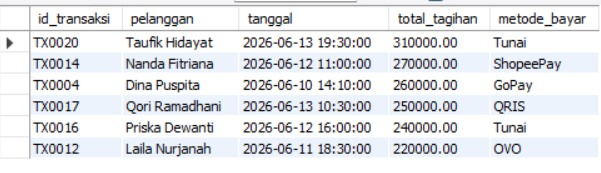
\includegraphics[width=0.85\linewidth]{query/output3.jpeg}
    \caption{Hasil Query Kasus 3 --- Transaksi di Atas Rp200.000}
    \label{fig:query3}
\end{figure}

\subsection{Kasus 4: Rekap Penjualan Produk Kantin per Kategori}

Kasus ini menghasilkan laporan produk kantin paling laris berdasarkan total kuantitas terjual per kategori. \textit{Query} menggunakan operasi agregasi \texttt{SUM} dan \texttt{GROUP BY} setelah menggabungkan tabel \texttt{produk\_kantin\_transaksi}, \texttt{produk\_kantin}, dan \texttt{kategori}.

\begin{lstlisting}[style=sql, caption={Query Kasus 4 --- Rekap Penjualan Produk Kantin}, label={lst:query4}]
SELECT
    kt.nama_kategori                AS kategori,
    pk.nama_produk                  AS produk,
    SUM(pkt.qty)                    AS total_terjual,
    SUM(pkt.subtotal)               AS total_pendapatan
FROM produk_kantin_transaksi pkt
JOIN produk_kantin pk ON pkt.produk_kantin_id_produk = pk.id_produk
JOIN kategori      kt ON pk.kategori_id_kategori     = kt.id_kategori
WHERE pkt.qty > 0
GROUP BY kt.nama_kategori, pk.nama_produk
ORDER BY total_terjual DESC, total_pendapatan DESC;
\end{lstlisting}

\begin{figure}[H]
    \centering
    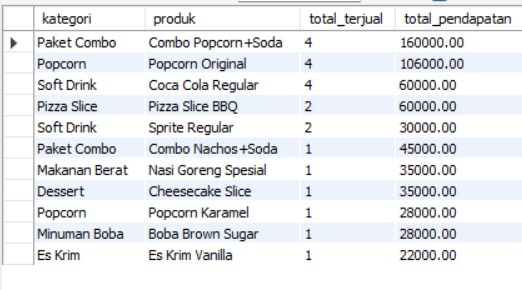
\includegraphics[width=0.85\linewidth]{query/output4.jpeg}
    \caption{Hasil Query Kasus 4 --- Rekap Penjualan Produk Kantin per Kategori}
    \label{fig:query4}
\end{figure}

\subsection{Kasus 5: Menampilkan Pelanggan yang Belum Pernah Bertransaksi}

Kasus ini menampilkan pelanggan terdaftar yang belum pernah melakukan transaksi sama sekali. \textit{Query} menggunakan operasi \textit{set difference} yang diimplementasikan dengan \texttt{NOT IN}, yaitu mengambil \texttt{id\_pelanggan} dari tabel \texttt{pelanggan} yang tidak terdapat pada kolom \texttt{pelanggan\_id\_pelanggan} di tabel \texttt{transaksi}.

\begin{lstlisting}[style=sql, caption={Query Kasus 5 --- Pelanggan Belum Pernah Bertransaksi}, label={lst:query5}]
SELECT
    pl.id_pelanggan         AS id_pelanggan,
    pl.nama_pelanggan       AS nama_pelanggan,
    pl.no_telp_pelanggan    AS nomor_telepon,
    pl.email_pelanggan      AS email
FROM pelanggan pl
WHERE pl.id_pelanggan NOT IN (
    SELECT DISTINCT tx.pelanggan_id_pelanggan
    FROM transaksi tx
    WHERE tx.pelanggan_id_pelanggan IS NOT NULL
)
ORDER BY pl.id_pelanggan;
\end{lstlisting}

\begin{figure}[H]
    \centering
    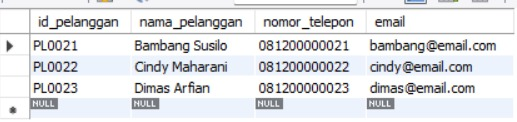
\includegraphics[width=0.85\linewidth]{query/output5.jpeg}
    \caption{Hasil Query Kasus 5 --- Pelanggan Belum Pernah Bertransaksi}
    \label{fig:query5}
\end{figure}

\clearpage

% ============================================================
% SECTION 6: SQL FUNCTIONS
% ============================================================
\section{Implementasi SQL \textit{Function}}

Implementasi dilakukan pada basis data \texttt{MBD\_FP} yang terdiri dari 18 tabel utama sesuai PDM. Tiga \textit{function} berikut dibuat untuk memenuhi kebutuhan kalkulasi otomatis dalam operasional bioskop CineTrack. Setiap \textit{function} bersifat \texttt{DETERMINISTIC} dan \texttt{READS SQL DATA}, artinya selalu menghasilkan nilai yang sama untuk input yang sama dan tidak memodifikasi data.

\subsection{\textit{Function} 1: \texttt{GetTotalTiketByPelanggan}}

\textit{Function} pertama bertujuan untuk mengembalikan jumlah tiket yang pernah dibeli oleh seorang pelanggan berdasarkan \texttt{id\_pelanggan} yang diberikan sebagai parameter input. \textit{Function} ini melakukan operasi \texttt{COUNT} dengan JOIN antara tabel \texttt{tiket} dan \texttt{transaksi}, kemudian mengembalikan hasilnya sebagai nilai \texttt{INT}.

\textbf{Skenario:} Tim loyalitas CineTrack ingin mengetahui seberapa sering seorang pelanggan membeli tiket agar dapat menentukan \textit{threshold} reward program. Dengan memanggil \textit{function} ini menggunakan \texttt{id\_pelanggan}, sistem dapat langsung mengetahui total tiket yang pernah dipesan tanpa harus menulis ulang \textit{query} JOIN setiap saat.

\begin{lstlisting}[style=sql, caption={\textit{Function} 1 --- \texttt{GetTotalTiketByPelanggan}}, label={lst:func1}]
DELIMITER $$

CREATE FUNCTION GetTotalTiketByPelanggan(p_id_pelanggan CHAR(6))
RETURNS INT
DETERMINISTIC
READS SQL DATA
BEGIN
    DECLARE v_total INT;

    SELECT COUNT(tk.id_tiket)
    INTO   v_total
    FROM   tiket     tk
    JOIN   transaksi tx ON tk.transaksi_id_transaksi = tx.id_transaksi
    WHERE  tx.pelanggan_id_pelanggan = p_id_pelanggan;

    RETURN v_total;
END$$

DELIMITER ;

-- Contoh pemanggilan:
SELECT GetTotalTiketByPelanggan('PL0001') AS TotalTiket;
\end{lstlisting}

Parameter \texttt{p\_id\_pelanggan} merupakan parameter input bertipe \texttt{CHAR(6)} dengan prefiks \texttt{p\_} sebagai konvensi penamaan agar tidak ambigu dengan nama kolom tabel. Variabel \texttt{v\_total} dideklarasikan dengan \texttt{DECLARE} untuk menampung hasil \texttt{COUNT}, kemudian diisi menggunakan sintaks \texttt{SELECT INTO}. JOIN ke tabel \texttt{transaksi} diperlukan karena relasi antara \texttt{tiket} dan \texttt{pelanggan} bersifat tidak langsung, melainkan melalui entitas \texttt{transaksi}.

\begin{figure}[H]
    \centering
    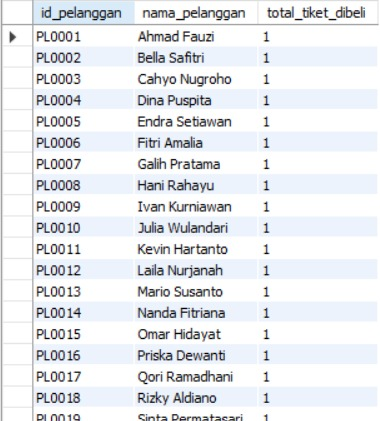
\includegraphics[width=0.6\linewidth]{function/output1.jpeg}
    \caption{Hasil Eksekusi \textit{Function} 1 --- \texttt{GetTotalTiketByPelanggan}}
    \label{fig:func1}
\end{figure}

\subsection{\textit{Function} 2: \texttt{GetPendapatanByStudio}}

\textit{Function} kedua bertujuan untuk menghitung total pendapatan tiket dari seluruh tiket yang terjual pada jadwal tayang di studio tertentu, berdasarkan \texttt{id\_studio} yang diberikan. \textit{Function} mengembalikan nilai \texttt{DECIMAL(12,2)} yang merepresentasikan total \texttt{harga\_beli} seluruh tiket di studio tersebut.

\textbf{Skenario:} Manajer operasional CineTrack ingin mengevaluasi performa setiap studio untuk keperluan laporan pendapatan harian. Dengan \textit{function} ini, sistem dapat langsung mengembalikan total pendapatan tiket per studio tanpa perlu melakukan JOIN manual ke \texttt{jadwal\_tayang} setiap kali laporan dibutuhkan. Apabila studio belum memiliki tiket terjual, \textit{function} mengembalikan \texttt{0.00} melalui \texttt{COALESCE}.

\begin{lstlisting}[style=sql, caption={\textit{Function} 2 --- \texttt{GetPendapatanByStudio}}, label={lst:func2}]
DELIMITER $$

CREATE FUNCTION GetPendapatanByStudio(p_id_studio CHAR(6))
RETURNS DECIMAL(12,2)
DETERMINISTIC
READS SQL DATA
BEGIN
    DECLARE v_total DECIMAL(12,2);

    SELECT COALESCE(SUM(tk.harga_beli), 0.00)
    INTO   v_total
    FROM   tiket          tk
    JOIN   jadwal_tayang  jt ON tk.jadwal_tayang_id_jadwal = jt.id_jadwal
    WHERE  jt.studio_id_studio = p_id_studio;

    RETURN v_total;
END$$

DELIMITER ;

-- Contoh pemanggilan:
SELECT GetPendapatanByStudio('ST0001') AS TotalPendapatan;
\end{lstlisting}

Penggunaan \texttt{COALESCE(SUM(...), 0.00)} memastikan \textit{function} tidak mengembalikan \texttt{NULL} ketika belum ada tiket terjual di studio tersebut. JOIN ke \texttt{jadwal\_tayang} diperlukan karena relasi \texttt{tiket} ke \texttt{studio} bersifat tidak langsung, melalui entitas \texttt{jadwal\_tayang} sebagai perantara.

\begin{figure}[H]
    \centering
    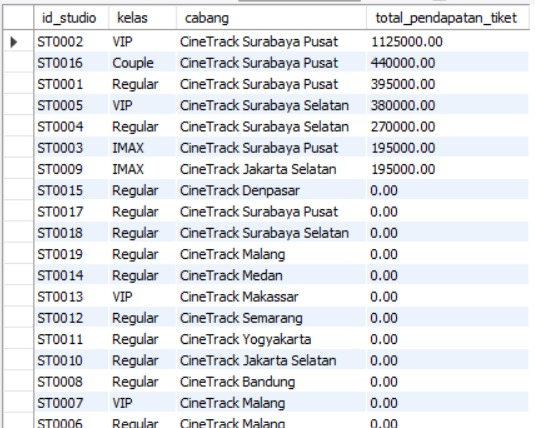
\includegraphics[width=0.6\linewidth]{function/output2.jpeg}
    \caption{Hasil Eksekusi \textit{Function} 2 --- \texttt{GetPendapatanByStudio}}
    \label{fig:func2}
\end{figure}

\subsection{\textit{Function} 3: \texttt{GetDurasiTayang}}

\textit{Function} ketiga bertujuan untuk mengembalikan durasi film (dalam menit) yang dijadwalkan pada sesi tayang tertentu berdasarkan \texttt{id\_jadwal} yang diberikan. \textit{Function} ini mengambil nilai \texttt{durasi} dari tabel \texttt{film} melalui relasi \texttt{jadwal\_tayang\_film}, dengan pengamanan \texttt{LIMIT 1} apabila satu jadwal memuat lebih dari satu film.

\textbf{Skenario:} Tim penjadwalan CineTrack perlu memastikan tidak ada tumpang tindih jadwal antar sesi. Dengan mengetahui durasi film dari \textit{function} ini, tim dapat menghitung estimasi jam selesai setiap sesi dan menentukan kapan sesi berikutnya dapat dimulai. \textit{Function} juga digunakan dalam \textit{query} gabungan yang menghitung \texttt{estimasi\_selesai} menggunakan \texttt{DATE\_ADD}.

\begin{lstlisting}[style=sql, caption={\textit{Function} 3 --- \texttt{GetDurasiTayang}}, label={lst:func3}]
DELIMITER $$

CREATE FUNCTION GetDurasiTayang(p_id_jadwal CHAR(6))
RETURNS INT
DETERMINISTIC
READS SQL DATA
BEGIN
    DECLARE v_durasi INT;

    SELECT f.durasi
    INTO   v_durasi
    FROM   jadwal_tayang_film jtf
    JOIN   film               f ON jtf.film_id_film = f.id_film
    WHERE  jtf.jadwal_tayang_id_jadwal = p_id_jadwal
    ORDER BY jtf.film_id_film
    LIMIT 1;

    RETURN COALESCE(v_durasi, 0);
END$$

DELIMITER ;

-- Contoh pemanggilan:
SELECT GetDurasiTayang('JD0001') AS DurasiMenit;

-- Query gabungan dengan estimasi jam selesai:
SELECT
    jt.id_jadwal,
    jt.waktu_tayang                                     AS mulai,
    f.judul                                             AS film,
    GetDurasiTayang(jt.id_jadwal)                       AS durasi_menit,
    DATE_ADD(jt.waktu_tayang,
        INTERVAL GetDurasiTayang(jt.id_jadwal) MINUTE)  AS estimasi_selesai
FROM jadwal_tayang      jt
JOIN jadwal_tayang_film jtf ON jt.id_jadwal         = jtf.jadwal_tayang_id_jadwal
JOIN film               f   ON jtf.film_id_film     = f.id_film
ORDER BY jt.waktu_tayang;
\end{lstlisting}

Penggunaan \texttt{COALESCE(v\_durasi, 0)} memastikan \textit{function} tidak mengembalikan \texttt{NULL} ketika jadwal tidak memiliki film yang terdaftar. Klausa \texttt{ORDER BY jtf.film\_id\_film LIMIT 1} memastikan konsistensi hasil apabila satu jadwal memiliki lebih dari satu entri pada tabel junction \texttt{jadwal\_tayang\_film}.

\begin{figure}[H]
    \centering
    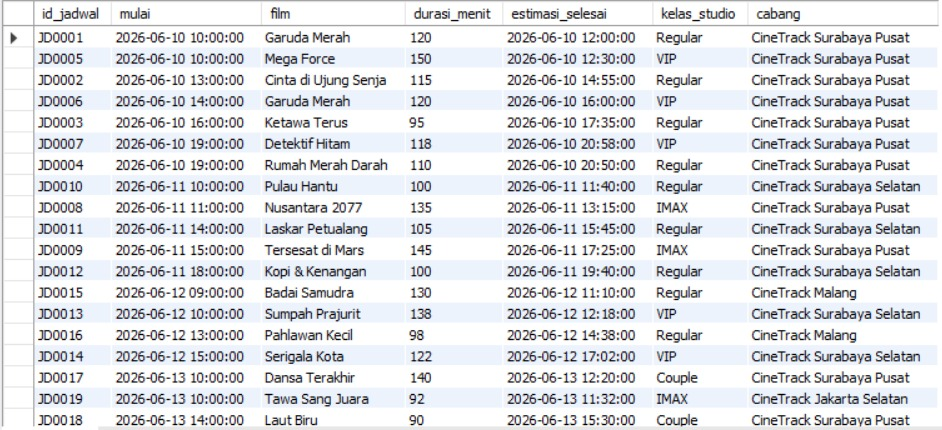
\includegraphics[width=0.6\linewidth]{function/output3.jpeg}
    \caption{Hasil Eksekusi \textit{Function} 3 --- \texttt{GetDurasiTayang}}
    \label{fig:func3}
\end{figure}

\clearpage

% ============================================================
% SECTION 7: STORED PROCEDURE (DIKERJAKAN OLEH ANGGOTA LAIN)
% ============================================================
\section{Implementasi \textit{Stored Procedure}}

\textit{Stored Procedure} merupakan sekumpulan perintah SQL yang disimpan langsung di dalam server basis data. Kegunaan utamanya adalah untuk menghemat waktu penulisan, mempercepat eksekusi perintah yang berulang, dan mempermudah eksekusi proses bisnis yang kompleks.

\subsection{Kasus 1: \textit{NaikkanHargaInflasi}}
Negara tempat CineTrack didirikan sering mengalami inflasi besar-besaran. Untuk itu, dibuat sebuah \textit{procedure} yang mempermudah para karyawan untuk mengganti semua harga tiket dan makanan secara massal tanpa harus memperbarui data satu per satu secara manual.

\begin{lstlisting}[style=sql, caption={\textit{Procedure} 1 --- \texttt{NaikkanHargaInflasi}}, label={lst:proc1}]
DELIMITER $$
CREATE PROCEDURE NaikkanHargaInflasi(IN p_persentase DECIMAL(5,2))
BEGIN
    UPDATE jadwal_tayang
    SET harga_dasar = harga_dasar + (harga_dasar * (p_persentase / 100));
    UPDATE produk_kantin
    SET harga_satuan = harga_satuan + (harga_satuan * (p_persentase / 100));
END$$
DELIMITER ;
\end{lstlisting}

\textit{Procedure} ini dipanggil dengan menyertakan parameter persentase kenaikan. Sebagai contoh, eksekusi \texttt{CALL NaikkanHargaInflasi(10);} akan menaikkan seluruh harga item sebesar 10\%. Sistem akan otomatis mengkalkulasi dan menyimpan harga terbaru. Berikut adalah perbandingan data sebelum dan sesudah \textit{procedure} dieksekusi:

\begin{figure}[H]
    \centering
    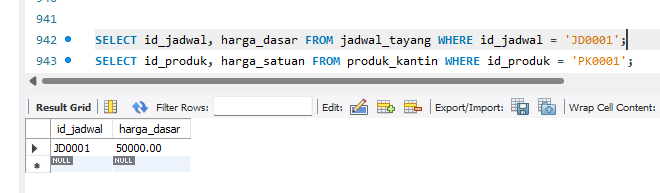
\includegraphics[width=0.6\linewidth]{procedure_image/before_inflasi.png}
    \caption{Harga Tiket Sebelum Eksekusi \texttt{NaikkanHargaInflasi}}
    \label{fig:proc1_tiket_before}
\end{figure}

\begin{figure}[H]
    \centering
    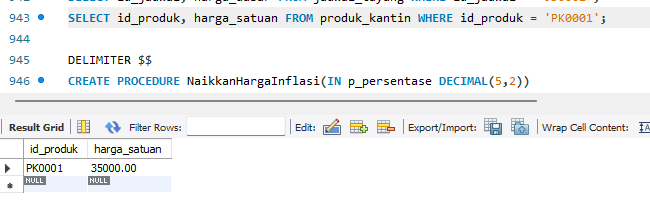
\includegraphics[width=0.6\linewidth]{procedure_image/before_inflasi(2).png}
    \caption{Harga Makanan Sebelum Eksekusi \texttt{NaikkanHargaInflasi}}
    \label{fig:proc1_food_before}
\end{figure}

\begin{figure}[H]
    \centering
    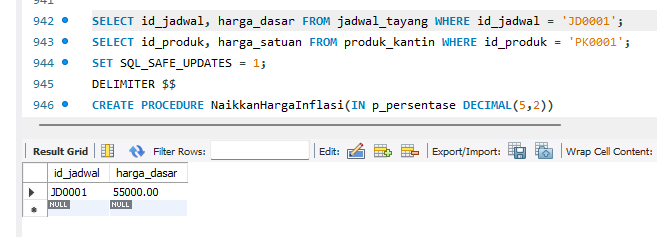
\includegraphics[width=0.6\linewidth]{procedure_image/ticket_after.png}
    \caption{Harga Tiket Sesudah Eksekusi \texttt{NaikkanHargaInflasi}}
    \label{fig:proc1_tiket_after}
\end{figure}

\begin{figure}[H]
    \centering
    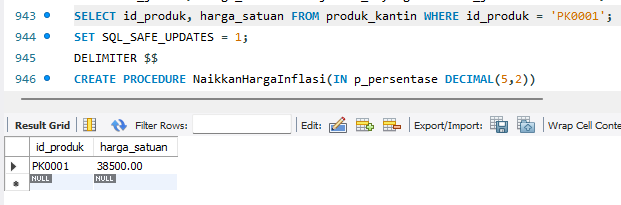
\includegraphics[width=0.6\linewidth]{procedure_image/food_after.png}
    \caption{Harga Makanan Sesudah Eksekusi \texttt{NaikkanHargaInflasi}}
    \label{fig:proc1_food_after}
\end{figure}


\subsection{Kasus 2: \textit{TambahJadwalMidnight}}
Seringkali manajer bioskop perlu menambah jadwal tayang ekstra pada tengah malam secara mendadak jika sebuah film sedang populer. \textit{Procedure} ini mengotomatiskan pembuatan ID jadwal baru, mengatur waktu tayang tepat pada pukul 23:30, dan langsung menghubungkannya ke tabel \textit{junction} \texttt{jadwal\_tayang\_film}.

\begin{lstlisting}[style=sql, caption={\textit{Procedure} 2 --- \texttt{TambahJadwalMidnight}}, label={lst:proc2}]
DELIMITER $$
CREATE PROCEDURE TambahJadwalMidnight(
    IN p_tanggal DATE, 
    IN p_harga_dasar DECIMAL(10,2), 
    IN p_id_studio CHAR(6), 
    IN p_id_film CHAR(6)
)
BEGIN
    DECLARE v_last_id CHAR(6);
    DECLARE v_next_id CHAR(6);
    DECLARE v_next_num INT;
    DECLARE v_waktu_tayang DATETIME;

    SELECT id_jadwal INTO v_last_id FROM jadwal_tayang ORDER BY id_jadwal DESC LIMIT 1;
    
    IF v_last_id IS NULL THEN
        SET v_next_id = 'JD0001';
    ELSE
        SET v_next_num = CAST(SUBSTRING(v_last_id, 3, 4) AS UNSIGNED) + 1;
        SET v_next_id = CONCAT('JD', LPAD(v_next_num, 4, '0'));
    END IF;

    SET v_waktu_tayang = CONCAT(p_tanggal, ' 23:30:00');

    INSERT INTO jadwal_tayang (id_jadwal, waktu_tayang, harga_dasar, studio_id_studio)
    VALUES (v_next_id, v_waktu_tayang, p_harga_dasar, p_id_studio);

    INSERT INTO jadwal_tayang_film (jadwal_tayang_id_jadwal, film_id_film)
    VALUES (v_next_id, p_id_film);
    
    SELECT v_next_id AS id_jadwal_midnight_baru;
END$$
DELIMITER ;
\end{lstlisting}

Gambar di bawah ini menunjukkan hasil \textit{output} setelah dilakukan pemanggilan \textit{procedure} tersebut, di mana sistem berhasil men-\textit{generate} ID jadwal baru untuk sesi penayangan tengah malam.

\begin{figure}[H]
    \centering
    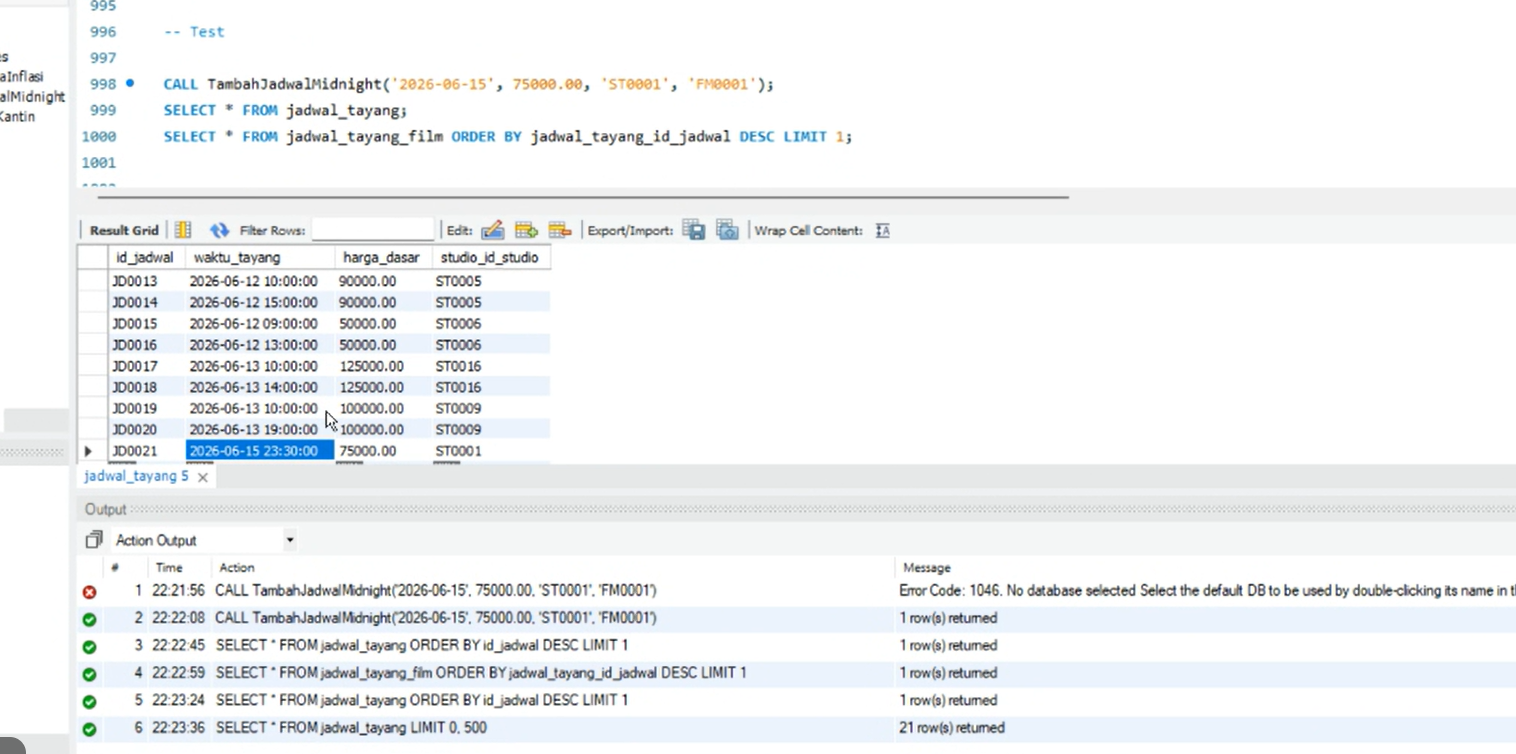
\includegraphics[width=0.6\linewidth]{procedure_image/Tambah_Jadwal.png}
    \caption{Hasil Eksekusi \texttt{TambahJadwalMidnight}}
    \label{fig:proc2_result}
\end{figure}


\subsection{Kasus 3: \textit{TambahStokKantin}}
Untuk mempermudah staf gudang saat menerima pengiriman barang baru dari \textit{supplier}, \textit{procedure} ini dibuat untuk langsung menambahkan kuantitas stok produk kantin berdasarkan ID produk yang diinputkan.

\begin{lstlisting}[style=sql, caption={\textit{Procedure} 3 --- \texttt{TambahStokKantin}}, label={lst:proc3}]
DELIMITER $$
CREATE PROCEDURE TambahStokKantin(IN p_id_produk CHAR(6), IN p_jumlah_tambah INT)
BEGIN
    UPDATE produk_kantin
    SET stok = stok + p_jumlah_tambah
    WHERE id_produk = p_id_produk;
END$$
DELIMITER ;
\end{lstlisting}

Gambar berikut menunjukkan perbandingan data stok produk kantin sebelum dan sesudah \textit{procedure} dijalankan. Dengan memberikan parameter ID produk dan jumlah barang baru, stok lama di dalam sistem akan otomatis terakumulasi.

\begin{figure}[H]
    \centering
    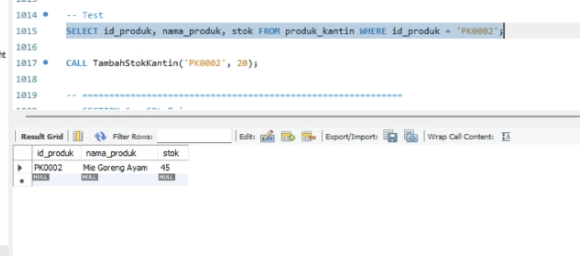
\includegraphics[width=0.6\linewidth]{procedure_image/before_call_kasus 3.png}
    \caption{Stok Kantin Sebelum Eksekusi \texttt{TambahStokKantin}}
    \label{fig:proc3_before}
\end{figure}

\begin{figure}[H]
    \centering
    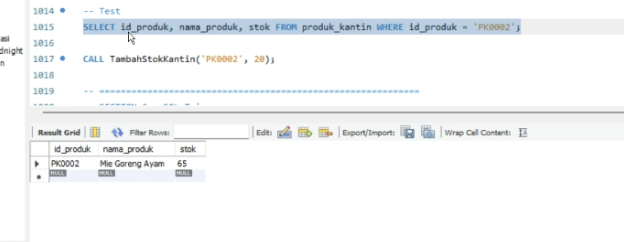
\includegraphics[width=0.6\linewidth]{procedure_image/after_call_kasus 3.png}
    \caption{Stok Kantin Sesudah Eksekusi \texttt{TambahStokKantin}}
    \label{fig:proc3_after}
\end{figure}


% TODO: Bagian ini dikerjakan oleh anggota kelompok lain.
% Struktur yang disarankan:
%
% \subsection{Deskripsi}
% Jelaskan tujuan stored procedure yang dibuat dalam konteks
% operasional CineTrack (misalnya: prosedur pembelian tiket,
% prosedur update stok kantin, dsb.)
%
% \subsection{Procedure 1: <NamaProcedure>}
% - Skenario kebutuhan
% - Kode SQL (gunakan \begin{lstlisting}[style=sql] ... \end{lstlisting})
% - Screenshot hasil eksekusi (gunakan \begin{figure}[H] ... \end{figure})
%
% \subsection{Procedure 2: <NamaProcedure>}
% (dst.)

\clearpage

% ============================================================
% SECTION 8: TRIGGERS
% ============================================================
\section{Implementasi \textit{Trigger}}
\textit{Trigger} merupakan kumpulan instruksi SQL yang berjalan secara otomatis sebagai reaksi atas suatu peristiwa (\textit{event}) INSERT, UPDATE, atau DELETE pada sebuah tabel. Pada sistem CineTrack, \textit{trigger} dimanfaatkan untuk menjaga integritas data dan mengotomatiskan kalkulasi operasional.

\subsection{Kasus 1: Pencegahan \textit{Double-Booking} Kursi}
Kasus pertama berfokus pada pencegahan redudansi pemesanan kursi. Sistem harus memastikan bahwa sebuah kursi pada jadwal tertentu tidak bisa dipesan lebih dari satu kali. \textit{Trigger} ini diatur untuk mengeksekusi pengecekan \texttt{BEFORE INSERT} pada tabel \texttt{tiket}.

\begin{lstlisting}[style=sql, caption={\textit{Trigger} 1 --- \texttt{Pencegahan Double Booking}}, label={lst:trg1}]
DELIMITER $$
CREATE TRIGGER trg_cegah_double_booking
BEFORE INSERT ON tiket
FOR EACH ROW
BEGIN
    DECLARE v_kursi_terisi INT;

    SELECT COUNT(*) INTO v_kursi_terisi
    FROM tiket
    WHERE jadwal_tayang_id_jadwal = NEW.jadwal_tayang_id_jadwal
      AND kursi_id_kursi = NEW.kursi_id_kursi;

    IF v_kursi_terisi > 0 THEN
        SIGNAL SQLSTATE '45000'
        SET MESSAGE_TEXT = 'Gagal: Kursi sudah dipesan untuk jadwal ini!';
    END IF;
END$$
DELIMITER ;
\end{lstlisting}

Apabila sistem mendeteksi bahwa kombinasi \texttt{id\_jadwal} dan \texttt{id\_kursi} yang diinputkan sudah ada di dalam tabel, maka \textit{trigger} akan membatalkan proses \textit{insert} dan memunculkan pesan \textit{error}. Berikut adalah hasil pengujiannya:

\begin{figure}[H]
    \centering
    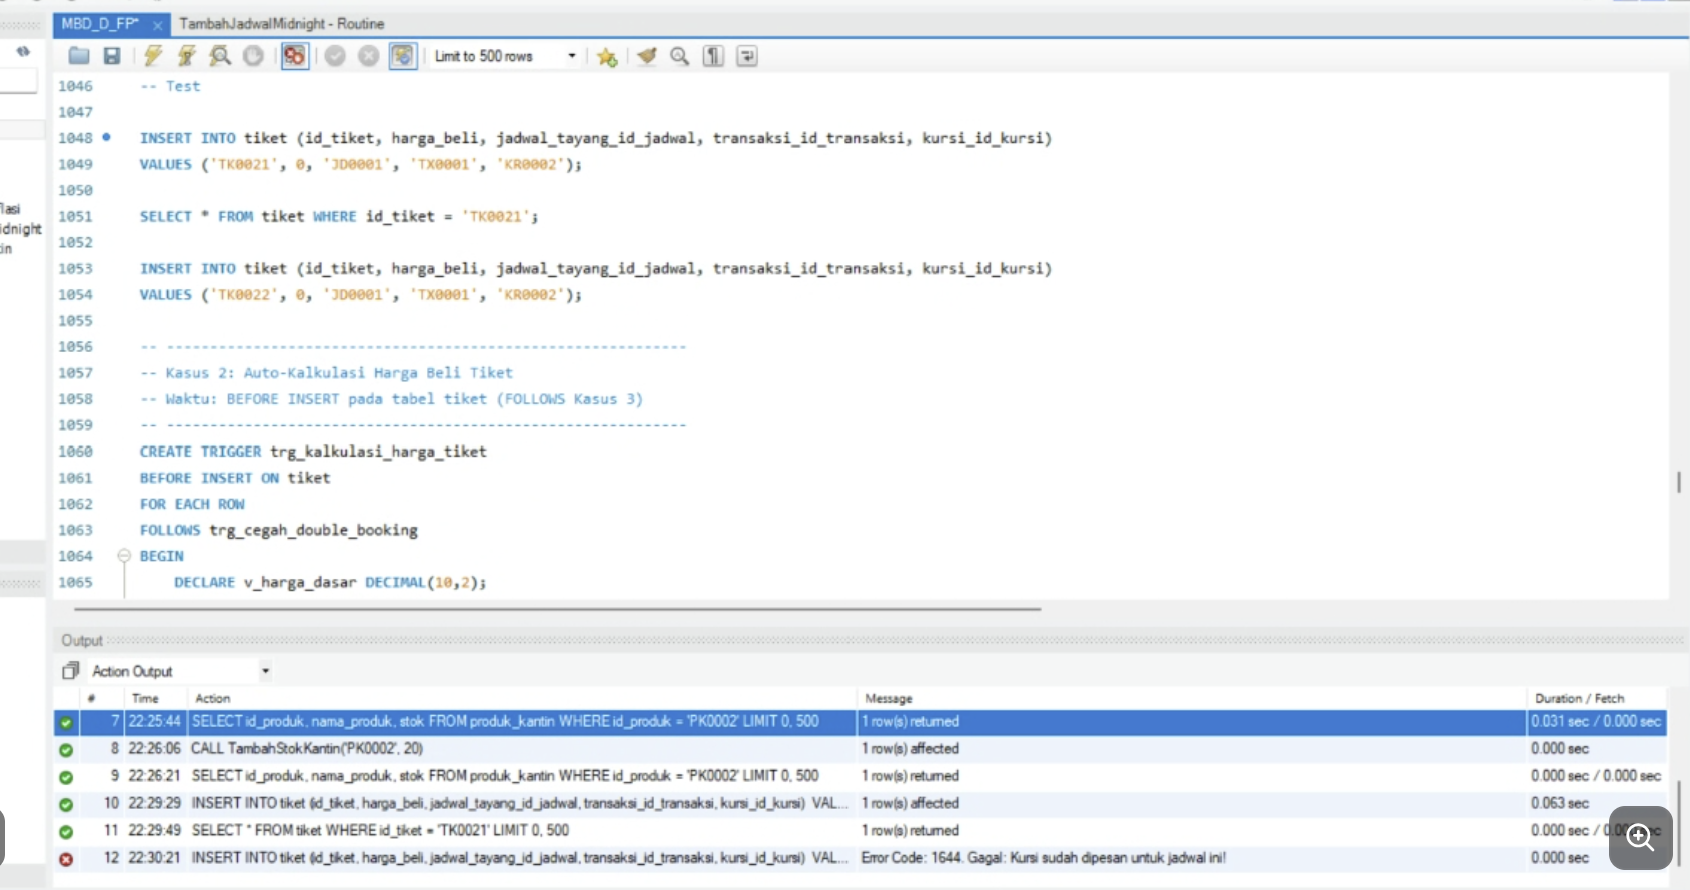
\includegraphics[width=0.6\linewidth]{trigger/kasus_1(1).png}
    \caption{Uji Coba \textit{Insert} Tiket Baru (Kondisi Berhasil)}
    \label{fig:trg1_test}
\end{figure}

\begin{figure}[H]
    \centering
    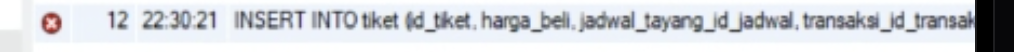
\includegraphics[width=0.6\linewidth]{trigger/kasus_1.png}
    \caption{Pesan \textit{Error} Saat Terjadi Indikasi \textit{Double Booking}}
    \label{fig:trg1_error}
\end{figure}


\subsection{Kasus 2: Auto-Kalkulasi Harga Beli Tiket}
Untuk meminimalisir kesalahan input (\textit{human error}) oleh staf, sistem dibuat agar dapat menghitung total harga tiket secara otomatis. \textit{Trigger} ini berjalan menggunakan klausa \texttt{FOLLOWS trg\_cegah\_double\_booking} agar kalkulasi harga hanya dilakukan setelah validasi ketersediaan kursi berhasil dilewati.

\begin{lstlisting}[style=sql, caption={\textit{Trigger} 2 --- \texttt{Auto-Kalkulasi Harga Beli}}, label={lst:trg2}]
DELIMITER $$
CREATE TRIGGER trg_kalkulasi_harga_tiket
BEFORE INSERT ON tiket
FOR EACH ROW
FOLLOWS trg_cegah_double_booking
BEGIN
    DECLARE v_harga_dasar DECIMAL(10,2);
    DECLARE v_tarif_tipe DECIMAL(10,2);

    SELECT harga_dasar INTO v_harga_dasar
    FROM jadwal_tayang
    WHERE id_jadwal = NEW.jadwal_tayang_id_jadwal;

    SELECT tarif_tipe INTO v_tarif_tipe
    FROM kursi
    WHERE id_kursi = NEW.kursi_id_kursi;

    SET NEW.harga_beli = v_harga_dasar + v_tarif_tipe;
END$$
DELIMITER ;
\end{lstlisting}

Proses ini mengambil harga dasar penayangan film dan menambahkannya dengan tarif tipe kursi yang dipilih, lalu menyimpannya ke atribut \texttt{harga\_beli}. Gambar di bawah ini menunjukkan harga yang terisi otomatis pada tabel tiket:

\begin{figure}[H]
    \centering
    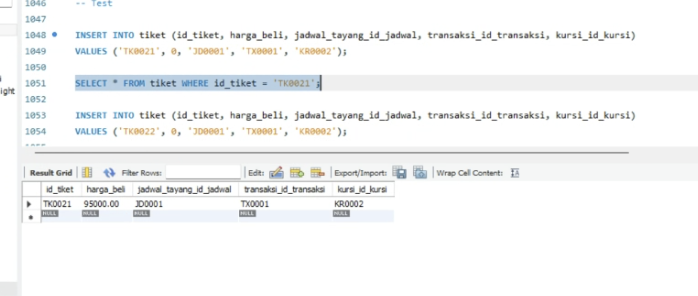
\includegraphics[width=0.6\linewidth]{trigger/kasus_2.png}
    \caption{Hasil Kalkulasi Otomatis Harga Tiket pada Basis Data}
    \label{fig:trg2_result}
\end{figure}


\subsection{Kasus 3: Pengurangan Stok Kantin Otomatis}
Kasus ketiga berfokus pada sinkronisasi data inventaris kantin. Ketika terjadi transaksi pembelian makanan atau minuman, stok di gudang harus diperbarui secara \textit{real-time}. \textit{Trigger} ini dieksekusi \texttt{AFTER INSERT} pada tabel \texttt{produk\_kantin\_transaksi}.

\begin{lstlisting}[style=sql, caption={\textit{Trigger} 3 --- \texttt{Pengurangan Stok Kantin}}, label={lst:trg3}]
DELIMITER $$
CREATE TRIGGER trg_kurangi_stok_kantin
AFTER INSERT ON produk_kantin_transaksi
FOR EACH ROW
BEGIN
    UPDATE produk_kantin
    SET stok = stok - NEW.qty
    WHERE id_produk = NEW.produk_kantin_id_produk;
END$$
DELIMITER ;
\end{lstlisting}

Begitu terdapat rekaman transaksi baru, sistem akan memotong jumlah \texttt{stok} di tabel master \texttt{produk\_kantin} sesuai dengan \texttt{qty} (kuantitas) barang yang dibeli oleh pelanggan. Berikut adalah perbandingan tabel produk sebelum dan sesudah transaksi terjadi:

\begin{figure}[H]
    \centering
    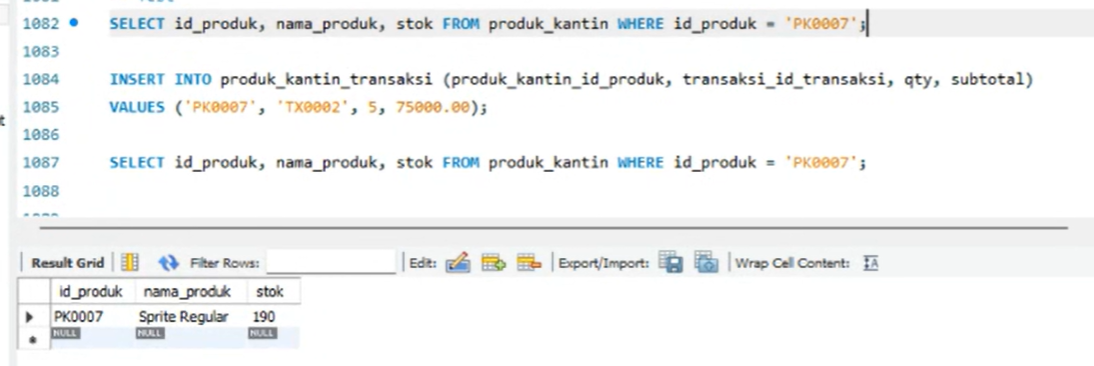
\includegraphics[width=0.6\linewidth]{trigger/kasus_3(1).png}
    \caption{Stok Produk Kantin Sebelum Terjadi Transaksi}
    \label{fig:trg3_before}
\end{figure}

\begin{figure}[H]
    \centering
    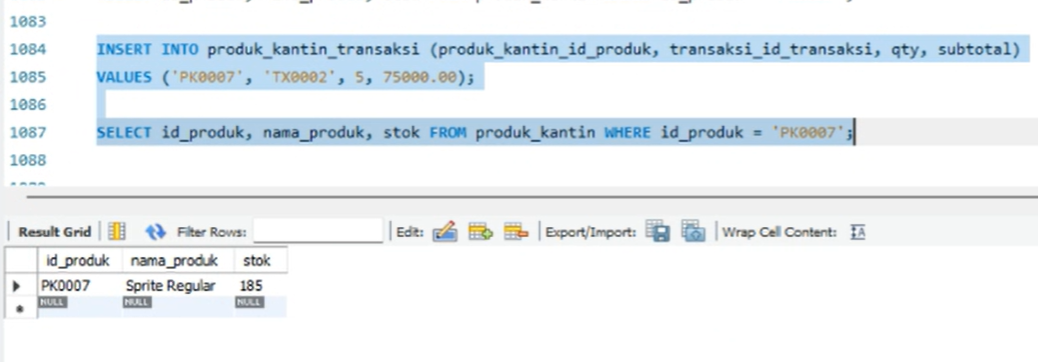
\includegraphics[width=0.6\linewidth]{trigger/kasus_3.png}
    \caption{Stok Produk Kantin Berkurang Secara Otomatis Setelah Transaksi}
    \label{fig:trg3_after}
\end{figure}

    
    



% TODO: Bagian ini dikerjakan oleh anggota kelompok lain.
% Struktur yang disarankan:
%
% \subsection{Deskripsi}
% Jelaskan tujuan trigger yang dibuat (misalnya: trigger untuk
% otomatis update stok produk kantin setelah transaksi,
% trigger untuk mencatat log perubahan harga, dsb.)
%
% \subsection{Trigger 1: <NamaTrigger>}
% - Skenario kebutuhan
% - Event: BEFORE/AFTER INSERT/UPDATE/DELETE pada tabel apa
% - Kode SQL
% - Screenshot hasil eksekusi
%
% \subsection{Trigger 2: <NamaTrigger>}
% (dst.)

\clearpage

% ============================================================
% SECTION 9: IMPLEMENTASI INDEXING
% Paste ini ke dalam \section{Implementasi \textit{Indexing}}
% di main.tex (gantikan blok % TODO yang ada)
% ============================================================

\section{Implementasi \textit{Indexing}}

\subsection{Deskripsi}

\textit{Indexing} adalah mekanisme struktur data tambahan yang memungkinkan MySQL menemukan baris yang relevan tanpa membaca seluruh isi tabel. Index bertipe BTREE menyimpan salinan kolom dalam bentuk terurut sehingga pencarian dapat dilakukan dalam kompleksitas $O(\log n)$ alih-alih $O(n)$.

Strategi \textit{indexing} pada CineTrack didasarkan pada frekuensi pemakaian kolom di seluruh komponen sistem: 5 \textit{query case}, 3 \textit{function}, 3 \textit{stored procedure}, dan 3 \textit{trigger}.

\begin{longtable}{|c|p{4.0cm}|p{2.8cm}|p{2.5cm}|p{3.2cm}|}
\caption{Daftar \textit{Index} pada Basis Data CineTrack}
\label{tab:daftar_index} \\
\hline
\textbf{No} & \textbf{Nama \textit{Index}} & \textbf{Tabel} & \textbf{Kolom} & \textbf{Digunakan Oleh} \\
\hline
\endfirsthead
\hline
\textbf{No} & \textbf{Nama \textit{Index}} & \textbf{Tabel} & \textbf{Kolom} & \textbf{Digunakan Oleh} \\
\hline
\endhead
\hline
\endlastfoot
1 & \texttt{\seqsplit{idx\_film\_status\_tayang}} & \texttt{film} & \texttt{status\_tayang} & Query Kasus 1 \\
\hline
2 & \texttt{\seqsplit{idx\_jtf\_film}} & \texttt{\seqsplit{jadwal\_tayang\_film}} & \texttt{film\_id\_film} & \textit{Function} 3, Query Kasus 2 \\
\hline
3 & \texttt{\seqsplit{idx\_transaksi\_total\_tagihan}} & \texttt{\seqsplit{transaksi}} & \texttt{total\_tagihan} & Query Kasus 3 \\
\hline
4 & \texttt{\seqsplit{idx\_jadwal\_waktu\_tayang}} & \texttt{jadwal\_tayang} & \texttt{waktu\_tayang} & Query Kasus 2, \textit{Function} 3, \textit{Procedure} 2 \\
\hline
\end{longtable}

\subsection{\textit{Index} 1: \texttt{idx\_film\_status\_tayang}}

\textbf{Skenario:} Query Kasus 1 memfilter tabel \texttt{film} dengan kondisi \texttt{WHERE status\_tayang = 'Now Showing'} untuk keperluan tim promosi. Kolom \texttt{status\_tayang} bukan bagian dari \textit{primary key} maupun \textit{foreign key}, sehingga tanpa index MySQL melakukan \textit{full table scan}. Index pada kolom ini memungkinkan MySQL langsung menunjuk baris yang relevan.

\begin{lstlisting}[style=sql, caption={\textit{Index} 1 --- \texttt{idx\_film\_status\_tayang}}, label={lst:idx1}]
CREATE INDEX idx_film_status_tayang
    ON film (status_tayang);

EXPLAIN
SELECT f.judul, f.status_tayang, g.nama_genre
FROM film f
JOIN film_genre fg ON f.id_film         = fg.film_id_film
JOIN genre      g  ON fg.genre_id_genre = g.id_genre
WHERE f.status_tayang = 'Now Showing'
ORDER BY f.judul, g.nama_genre;
\end{lstlisting}

\begin{figure}[H]
    \centering
    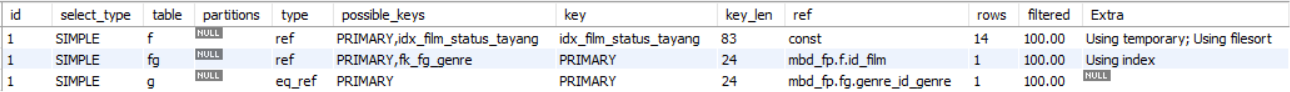
\includegraphics[width=1\linewidth]{index/output_idx1.png}
    \caption{Hasil \texttt{EXPLAIN} \textit{Index} 1}
    \label{fig:idx1}
\end{figure}

\subsection{\textit{Index} 2: \texttt{idx\_jtf\_film}}

\textbf{Skenario:} \textit{Primary key} tabel \textit{junction} \texttt{jadwal\_tayang\_film} adalah \textit{composite} (\texttt{jadwal\_tayang\_id\_jadwal}, \texttt{film\_id\_film}). Index BTREE pada PK \textit{composite} hanya efisien untuk \textit{lookup} yang dimulai dari kolom \textbf{pertama} (jadwal). Kolom kedua (\texttt{film\_id\_film}) tidak ter-\textit{cover} sebagai \textit{leading key}, sehingga \textit{reverse lookup}, yang digunakan oleh \textit{Function} \texttt{GetDurasiTayang} dan Query Kasus 2, tetap melakukan \textit{full scan} tanpa index ini.

\begin{lstlisting}[style=sql, caption={\textit{Index} 2 --- \texttt{idx\_jtf\_film}}, label={lst:idx2}]
CREATE INDEX idx_jtf_film
    ON jadwal_tayang_film (film_id_film);

EXPLAIN
SELECT jt.id_jadwal, jt.waktu_tayang, f.judul, f.durasi
FROM jadwal_tayang      jt
JOIN jadwal_tayang_film jtf ON jt.id_jadwal     = jtf.jadwal_tayang_id_jadwal
JOIN film               f   ON jtf.film_id_film = f.id_film
ORDER BY jt.waktu_tayang;
\end{lstlisting}

\begin{figure}[H]
    \centering
    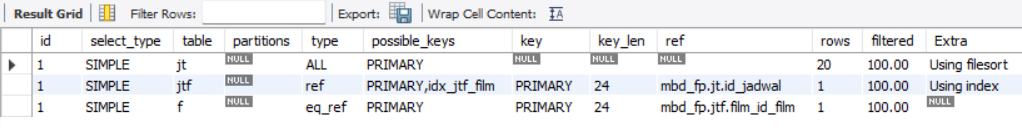
\includegraphics[width=1\linewidth]{index/output_idx2.png}
    \caption{Hasil \texttt{EXPLAIN} \textit{Index} 2}
    \label{fig:idx2}
\end{figure}

\subsection{\textit{Index} 3: \texttt{idx\_transaksi\_total\_tagihan}}

\textbf{Skenario:} Query Kasus 3 memfilter tabel \texttt{transaksi} dengan kondisi \texttt{WHERE total\_tagihan > 200000} untuk analisis transaksi bernilai tinggi. Kolom \texttt{total\_tagihan} bertipe \texttt{DECIMAL} dan tidak memiliki index apapun. Index pada kolom numerik menyimpan nilai secara terurut sehingga MySQL dapat langsung melompat ke nilai \textit{threshold} tanpa men-\textit{scan} seluruh tabel.

\begin{lstlisting}[style=sql, caption={\textit{Index} 3 --- \texttt{idx\_transaksi\_total\_tagihan}}, label={lst:idx3}]
CREATE INDEX idx_transaksi_total_tagihan
    ON transaksi (total_tagihan);

EXPLAIN
SELECT tx.id_transaksi, pl.nama_pelanggan,
       tx.total_tagihan, pb.metode_pembayaran
FROM transaksi  tx
JOIN pelanggan  pl ON tx.pelanggan_id_pelanggan   = pl.id_pelanggan
JOIN pembayaran pb ON tx.pembayaran_id_pembayaran = pb.id_pembayaran
WHERE tx.total_tagihan > 200000
ORDER BY tx.total_tagihan DESC;
\end{lstlisting}

\begin{figure}[H]
    \centering
    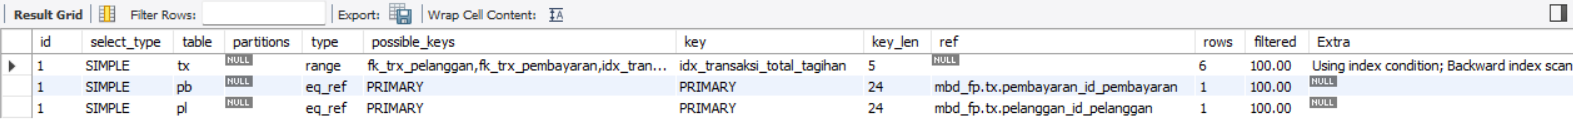
\includegraphics[width=1\linewidth]{index/output_idx3.png}
    \caption{Hasil \texttt{EXPLAIN} \textit{Index} 3}
    \label{fig:idx3}
\end{figure}

\subsection{\textit{Index} 4: \texttt{idx\_jadwal\_waktu\_tayang}}

\textbf{Skenario:} Kolom \texttt{waktu\_tayang} bertipe \texttt{DATETIME} diakses oleh tiga komponen sekaligus: Query Kasus 2 menggunakannya pada \texttt{ORDER BY}, \textit{Function} \texttt{GetDurasiTayang} (query gabungan) juga menggunakannya pada \texttt{ORDER BY}, dan \textit{Procedure} \texttt{TambahJadwalMidnight} membaca urutan jadwal terbaru. Tanpa index, setiap \texttt{ORDER BY} memaksa MySQL melakukan pengurutan di memori atau disk setelah \textit{full scan}. Index menyimpan \texttt{DATETIME} secara terurut sehingga \texttt{ORDER BY} dapat memanfaatkan \textit{index scan} langsung.

\begin{lstlisting}[style=sql, caption={\textit{Index} 4 --- \texttt{idx\_jadwal\_waktu\_tayang}}, label={lst:idx5}]
CREATE INDEX idx_jadwal_waktu_tayang
    ON jadwal_tayang (waktu_tayang);
    
EXPLAIN
SELECT jt.waktu_tayang, f.judul, st.kelas_studio,
       jt.harga_dasar, cb.nama_cabang
FROM jadwal_tayang      jt
JOIN jadwal_tayang_film jtf ON jt.id_jadwal        = jtf.jadwal_tayang_id_jadwal
JOIN film               f   ON jtf.film_id_film    = f.id_film
JOIN studio             st  ON jt.studio_id_studio = st.id_studio
JOIN cabang             cb  ON st.cabang_id_cabang = cb.id_cabang
ORDER BY jt.waktu_tayang;
\end{lstlisting}

\begin{figure}[H]
    \centering
    
\includegraphics[width=1\linewidth]{index/output_idx5.png}
    \caption{Hasil \texttt{EXPLAIN} \textit{Index} 4}
    \label{fig:idx5}
\end{figure}

\clearpage

\section{Demo Aplikasi Web CineTrack}
Demo web untuk mengimplementasikan fungsionalitas database secara utuh dapat dilihat pada link berikut: \url{https://its.id/m/CineTrack}

\section{Kesimpulan}
Berdasarkan perancangan dan implementasi yang telah dilakukan, dapat disimpulkan bahwa:
\begin{enumerate}
    \item \textbf{Perancangan Basis Data:} Sistem Basis Data CineTrack telah berhasil dirancang melalui tahapan Conceptual Data Model (CDM) dan Physical Data Model (PDM), serta telah dinormalisasi hingga Bentuk Normal Ketiga (3NF) guna mencegah redundansi dan anomali data.
    \item \textbf{Implementasi Fungsionalitas:} Seluruh aturan bisnis operasional bioskop telah diimplementasikan dengan sukses melalui 5 \textit{Query Cases} untuk pelaporan, 3 SQL \textit{Functions} untuk kalkulasi data baca, 3 \textit{Stored Procedures} untuk modifikasi massal, dan 3 \textit{Triggers} untuk otomatisasi seperti pencegahan \textit{double-booking} kursi.
    \item \textbf{Evaluasi dan Optimasi Kinerja:} Pembuatan \textit{Index} pada kolom-kolom yang sering digunakan untuk \textit{filtering} (WHERE) dan pengurutan (ORDER BY) terbukti secara signifikan meningkatkan kecepatan eksekusi \textit{query}, yang divalidasi melalui hasil \texttt{EXPLAIN}.
    \item \textbf{Pengujian dan Integrasi:} Keseluruhan sistem basis data telah berhasil diuji dan diintegrasikan secara \textit{Full-Stack} ke dalam aplikasi web CineTrack, yang membuktikan bahwa arsitektur basis data yang dibangun solid, responsif, dan siap digunakan untuk operasi bioskop berskala multi-cabang.
\end{enumerate}

\end{document}